\documentclass[11pt,a4paper]{scrreprt}
\usepackage[latin1]{inputenc}
\usepackage{enumerate}
\usepackage{verbatim}
\usepackage{moreverb}
\usepackage{subfigure}
\usepackage{graphicx}
\usepackage{amsmath}
\usepackage{amsfonts}
\newcommand{\field}[1]{\mathbb{#1}}
\usepackage{amssymb}
\usepackage{cite}
\usepackage{url}
\usepackage{listings}
%\usepackage{ngerman}
\usepackage{geometry}
\geometry{a4paper,left=30mm,right=30mm,top=35mm,bottom=25mm}

\pagestyle{headings}

\begin{document}
\title{Kangaroo \\ a mobile, location-aware task planer}
\author{Alexander Gutjahr \and Andreas Walz \and
        Daniel Schauenberg}

\maketitle

\tableofcontents

%introduction
\chapter{Introduction} % (fold)
\label{chp:introduction}
Kangaroo was developed as a team project at the Albert Ludwig University of
Freiburg. The goal was to develop an application which knows all events and
tasks data of a user. Based on this information, the best route to attend all
events and complete as many tasks as possible, is computed. In this document,
all information which was created during the development is collected.

Chapter 2 describes the requirements as defined by the Lehrstuhl, as well as the
resulting development goals and the abstract system structure that was designed
to fulfill these requirements.

Chapter 3 contains information about project planning and the development
process. This means the initial and refined project plan as well as the
description of the development process.

The process of evaluating suitable platforms is described in chapter 4. The main
focus here lies on the three mobile Operating Systems iPhone OS, Android and
Windows Mobile. Others are also described briefly. Additionally the decision
which routing engine to use is described in this chapter, too.

The actual development process is the focus of chapter 5. Here the platform
specifics, which impact the system design, are explained. Furthermore the main
parts of the application, as well as some important implementation details and
caveats are discussed.

The last chapter then provides a summary of the work with some reflections on
the completed work as well as an outlook, how to use this for future
development.


%definition of project scope
\chapter{Definition of project scope} % (fold)
	%external requirements
	\section{External requirements} % (fold)
	\label{chp:requirements}
	TODO: Introduce process  of requirement refinement: external (from klaus) --> internal (resulting rev. goals) --> appropriate system design and dev. process

TODO: outline the requirements from Klaus

\begin{figure}[h!]
\centering
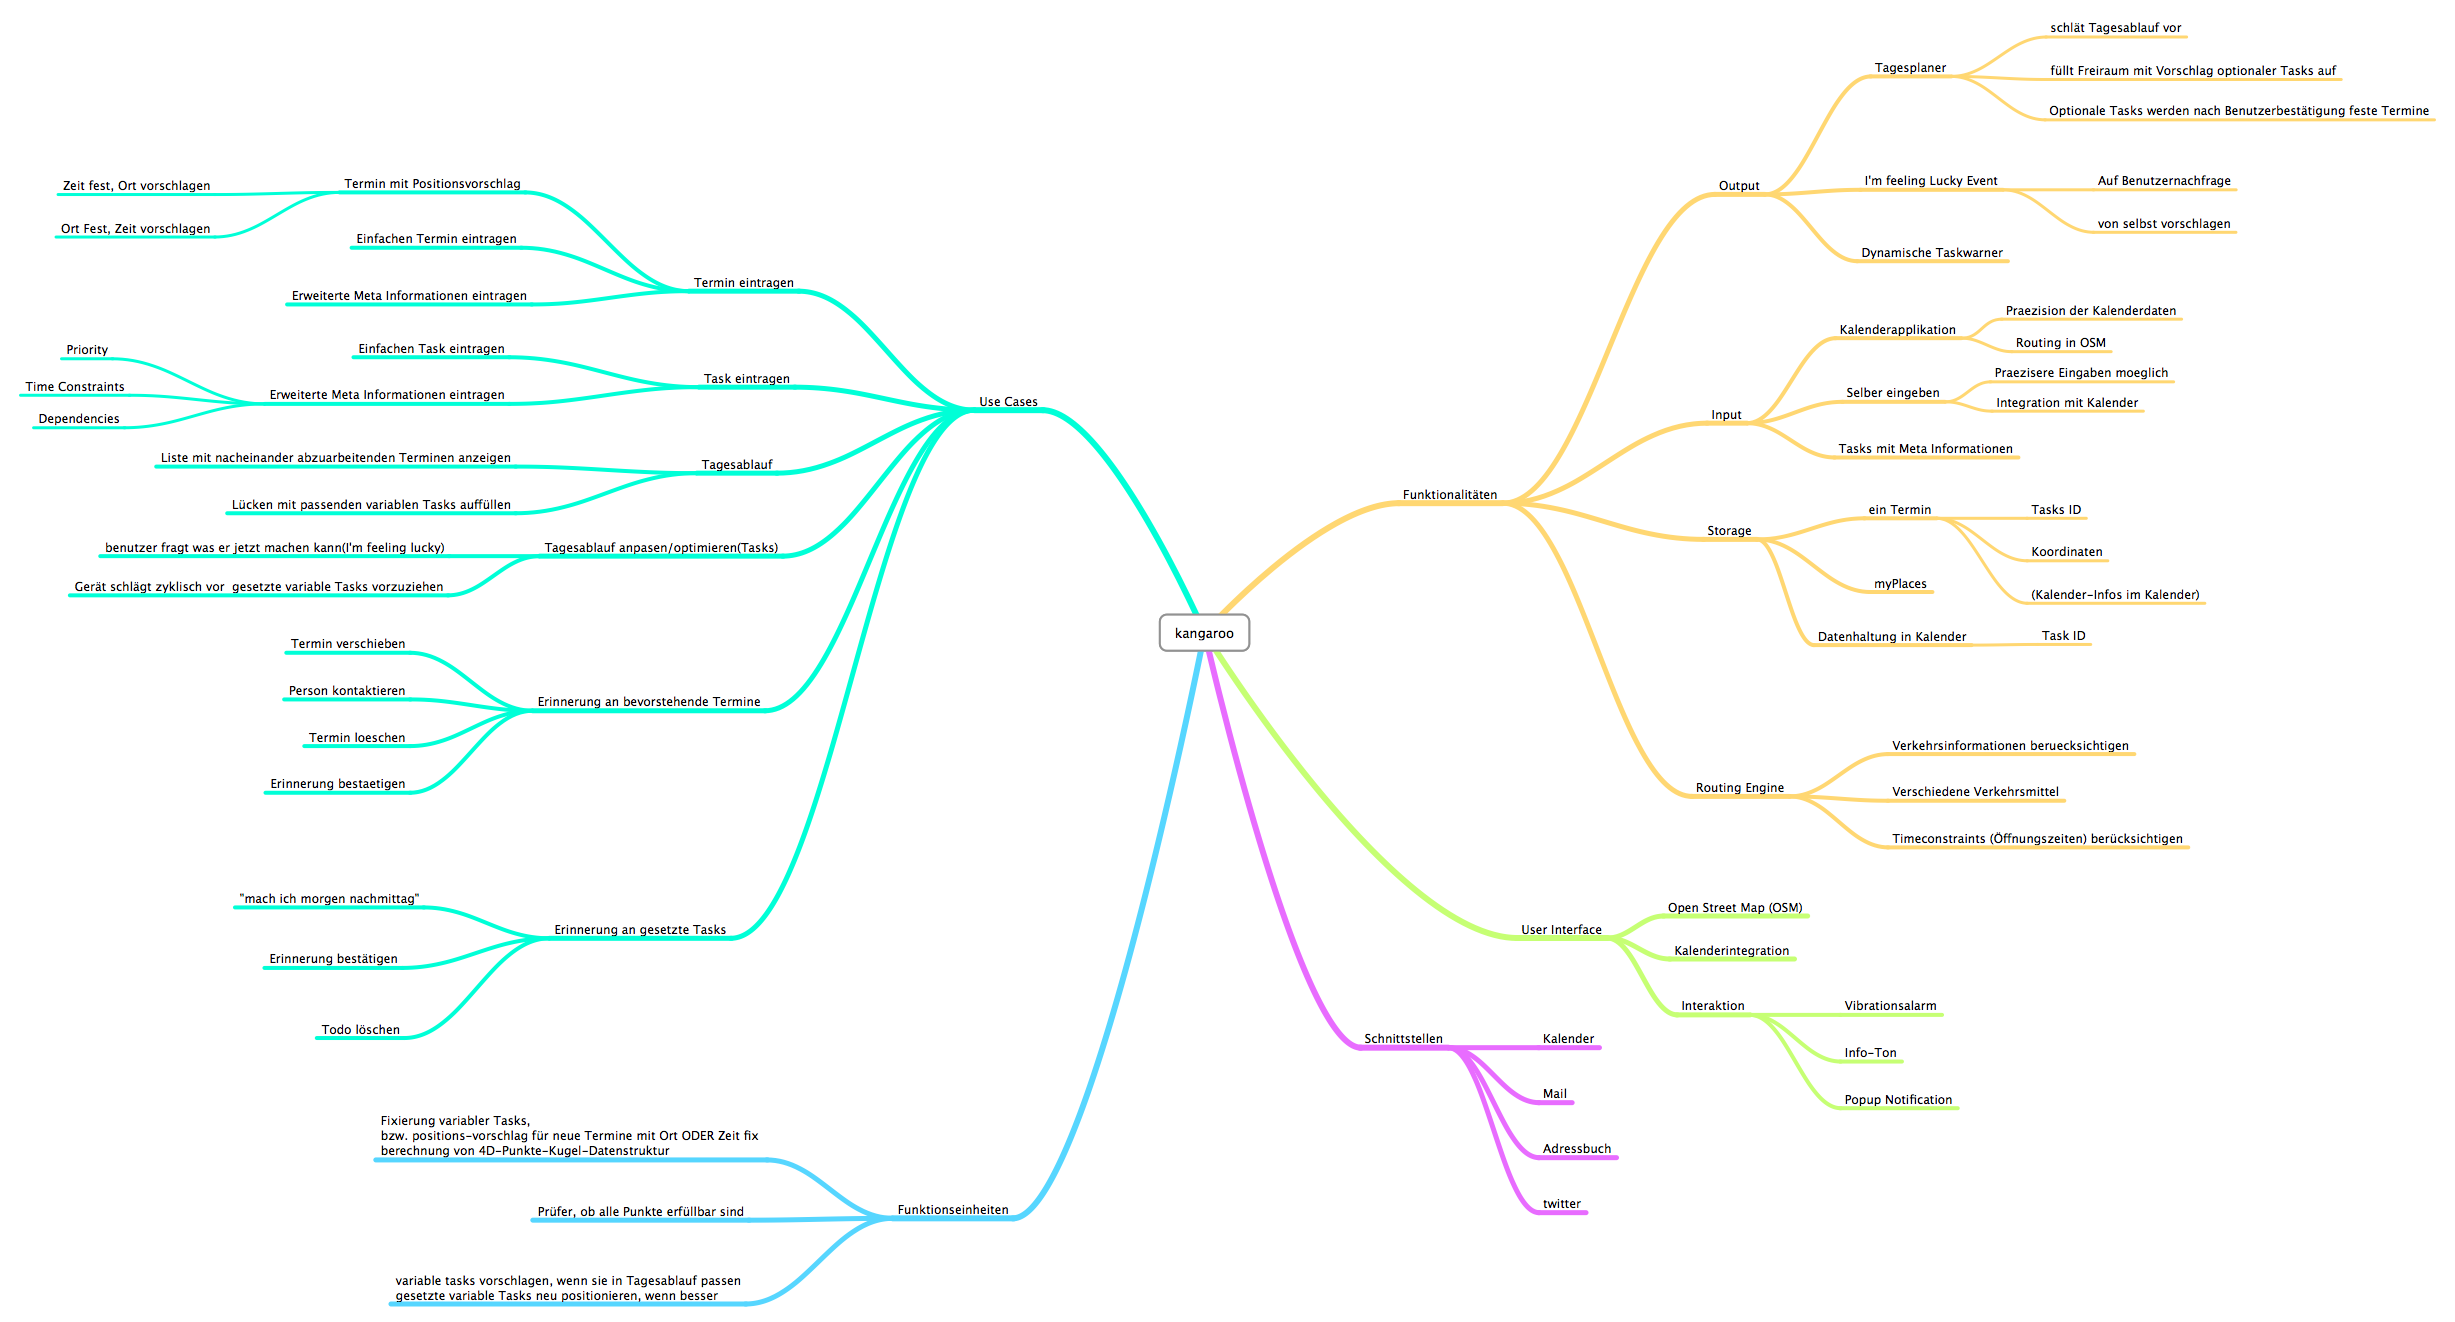
\includegraphics[width=16cm]{pics/kangaroo.png}
\caption{Mindmap with project goals, requirements and elements}
\label{mindmap}
\end{figure}
	
	%resulting dev. goals
	\section{Resulting development goals} % (fold)
	\label{chp:dev_goals}
	TODO: describe deve goals that result from the external requirements
	
	%abstract system design
	\section{Abstract System Structure} % (fold)
	\label{chp:structure}
	As stated in chapter \ref{chp:dev_goals}  one goal for the project is the creation of system structure with a formal and clean development process. One aspect of this approach is the creation of an abstract system structure before any considerations towards the platform or the implementation details have been made. The sole basis for the system structure shown in this chapter are the requirements listed in the chapters \ref{chp:requirements} and \ref{chp:dev_goals}.\\
Figure \ref{high_level_design} describes  the high level structure of the system. The design should be self explanatory. It implements the classical software paradigm of a distinction between three main system parts: user interface, application logic and data-storage. Note that all platform specific calls and interaction are abstracted through the data-storage module. The application-logic module doesn't need any information about the platform itself. 
\begin{figure}[h!]
\centering
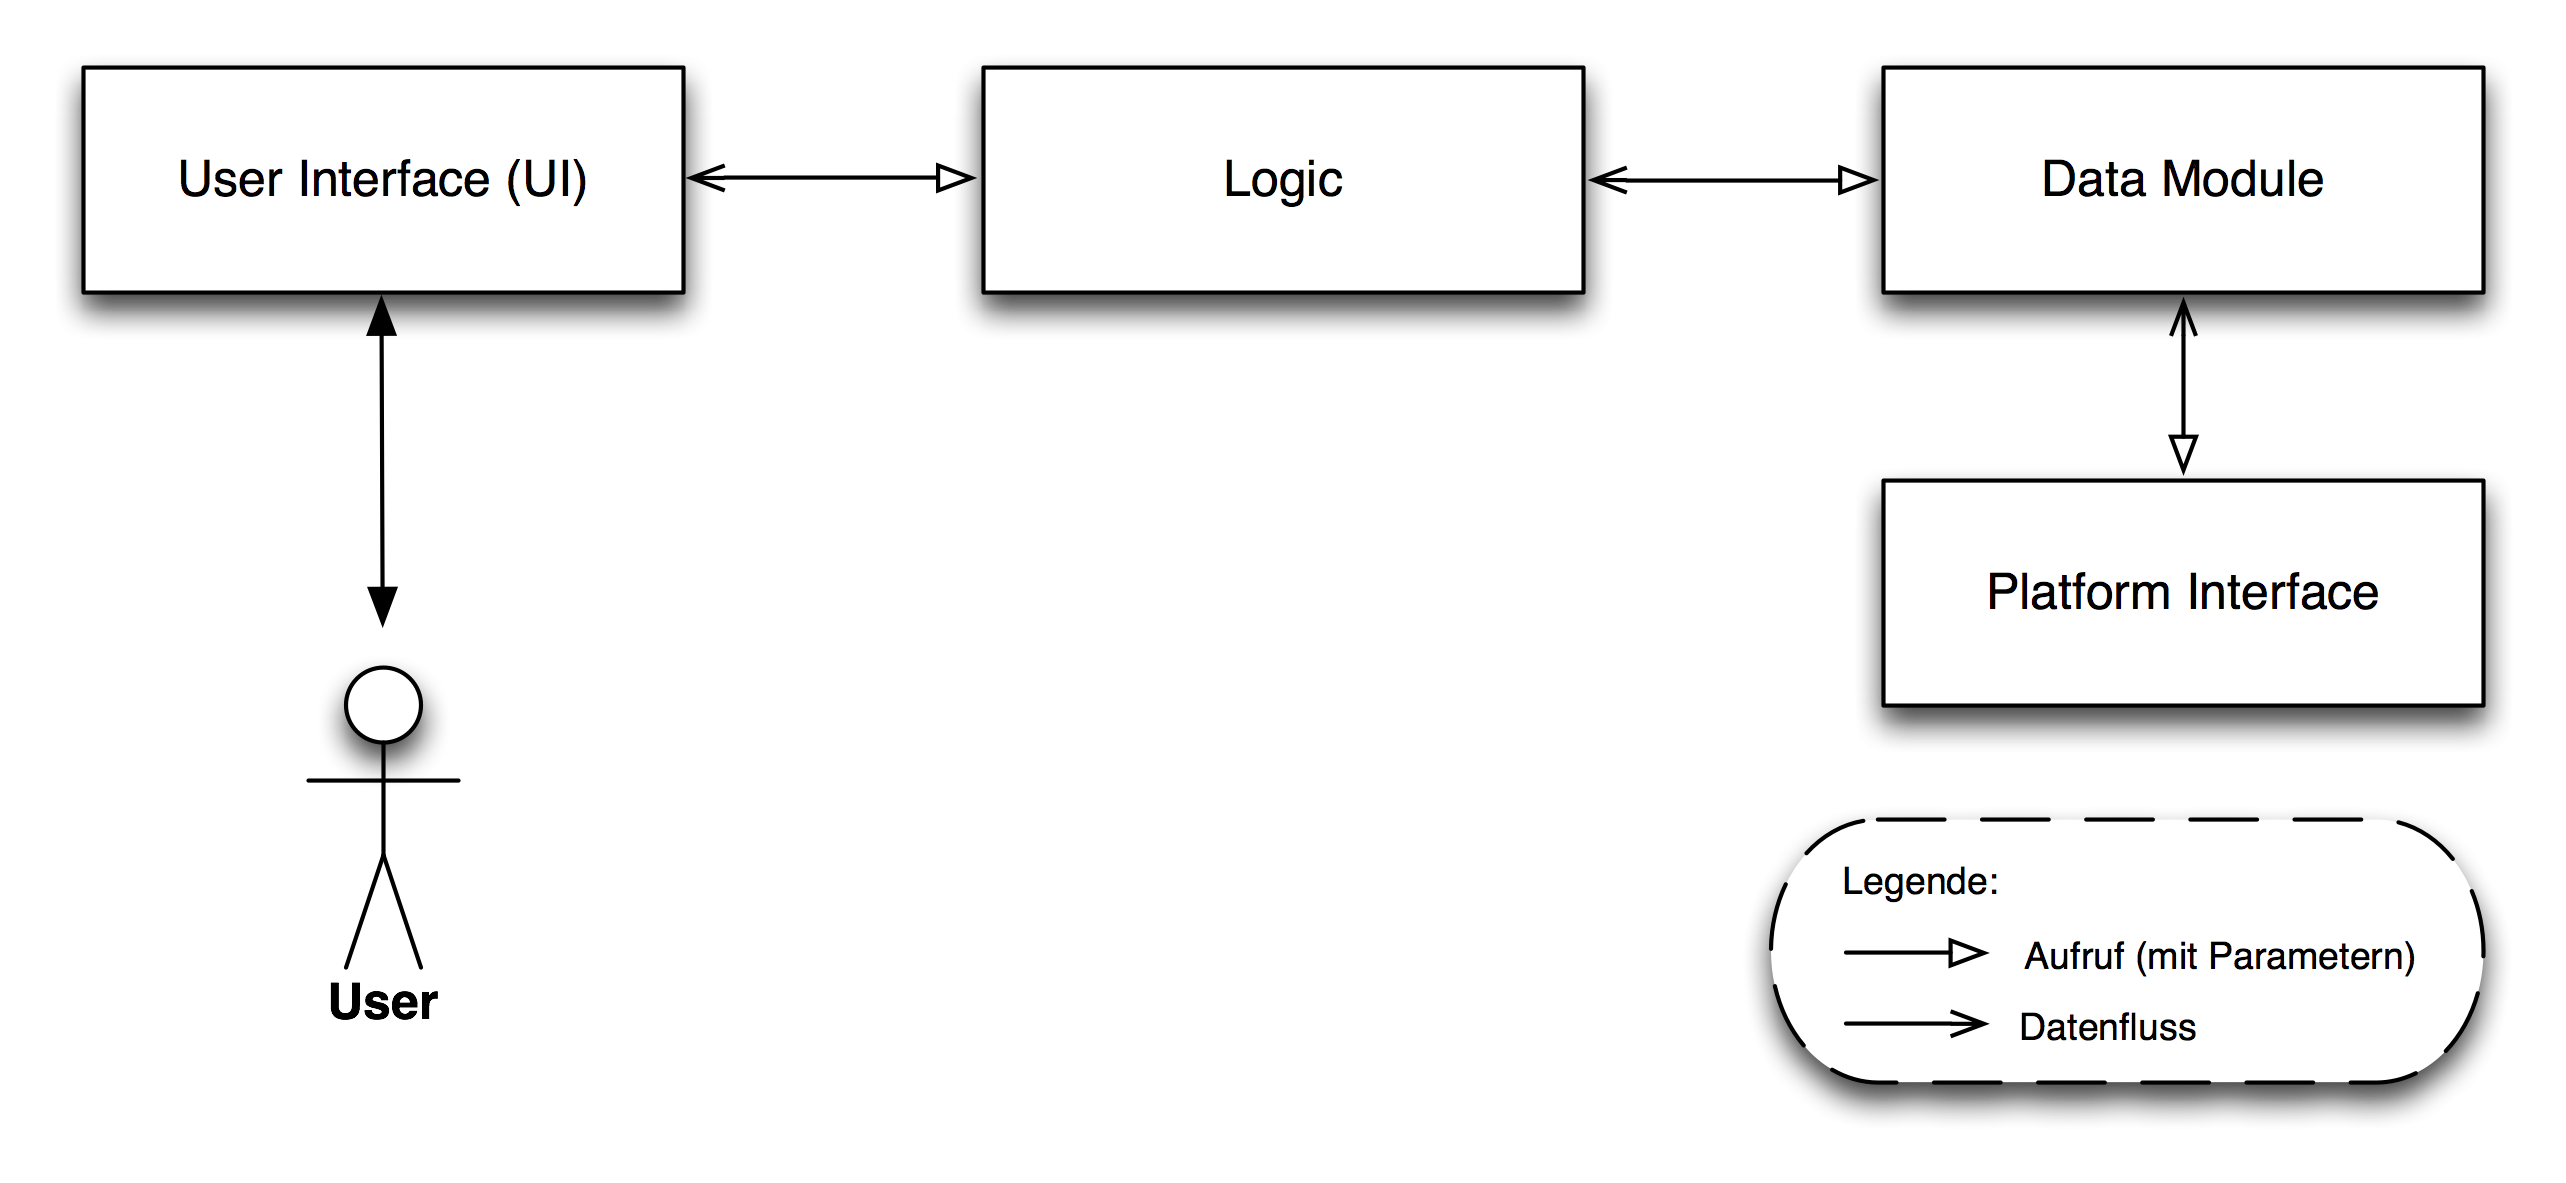
\includegraphics[width=16cm]{pics/top_level_design.png}
\caption{High level design of the system components}
\label{high_level_design}
\end{figure}
In figure \ref{logic} the inner structure of the application-logic is described. The sub-systems shown here are:
\begin{itemize}
\item Event Stuff: This module contains the main functionality of the software. It is described in details in figure \ref{event_stuff}.
\item Event Stuff Tools: This is a collection of helper-functions that solve common tasks for the Event Stuff module.
\item Routing: The routing engine and map-data management are located in this module, separated from the Event Stuff to reduce complexity and to impose the necessity to define clean interface between these system-parts
\item UI Manager: This as an Abstraction of the concrete implementation of the user interface. The Event Stuff module tells the UI-Manager about events that occur and the  UI Manager decides wether and how the user is to be made aware of the situation. With this abstraction the application can look and behave in completely different ways depending an the runtime-configuration of the UI Manager.  
\end{itemize}
\begin{figure}[h!]
\centering
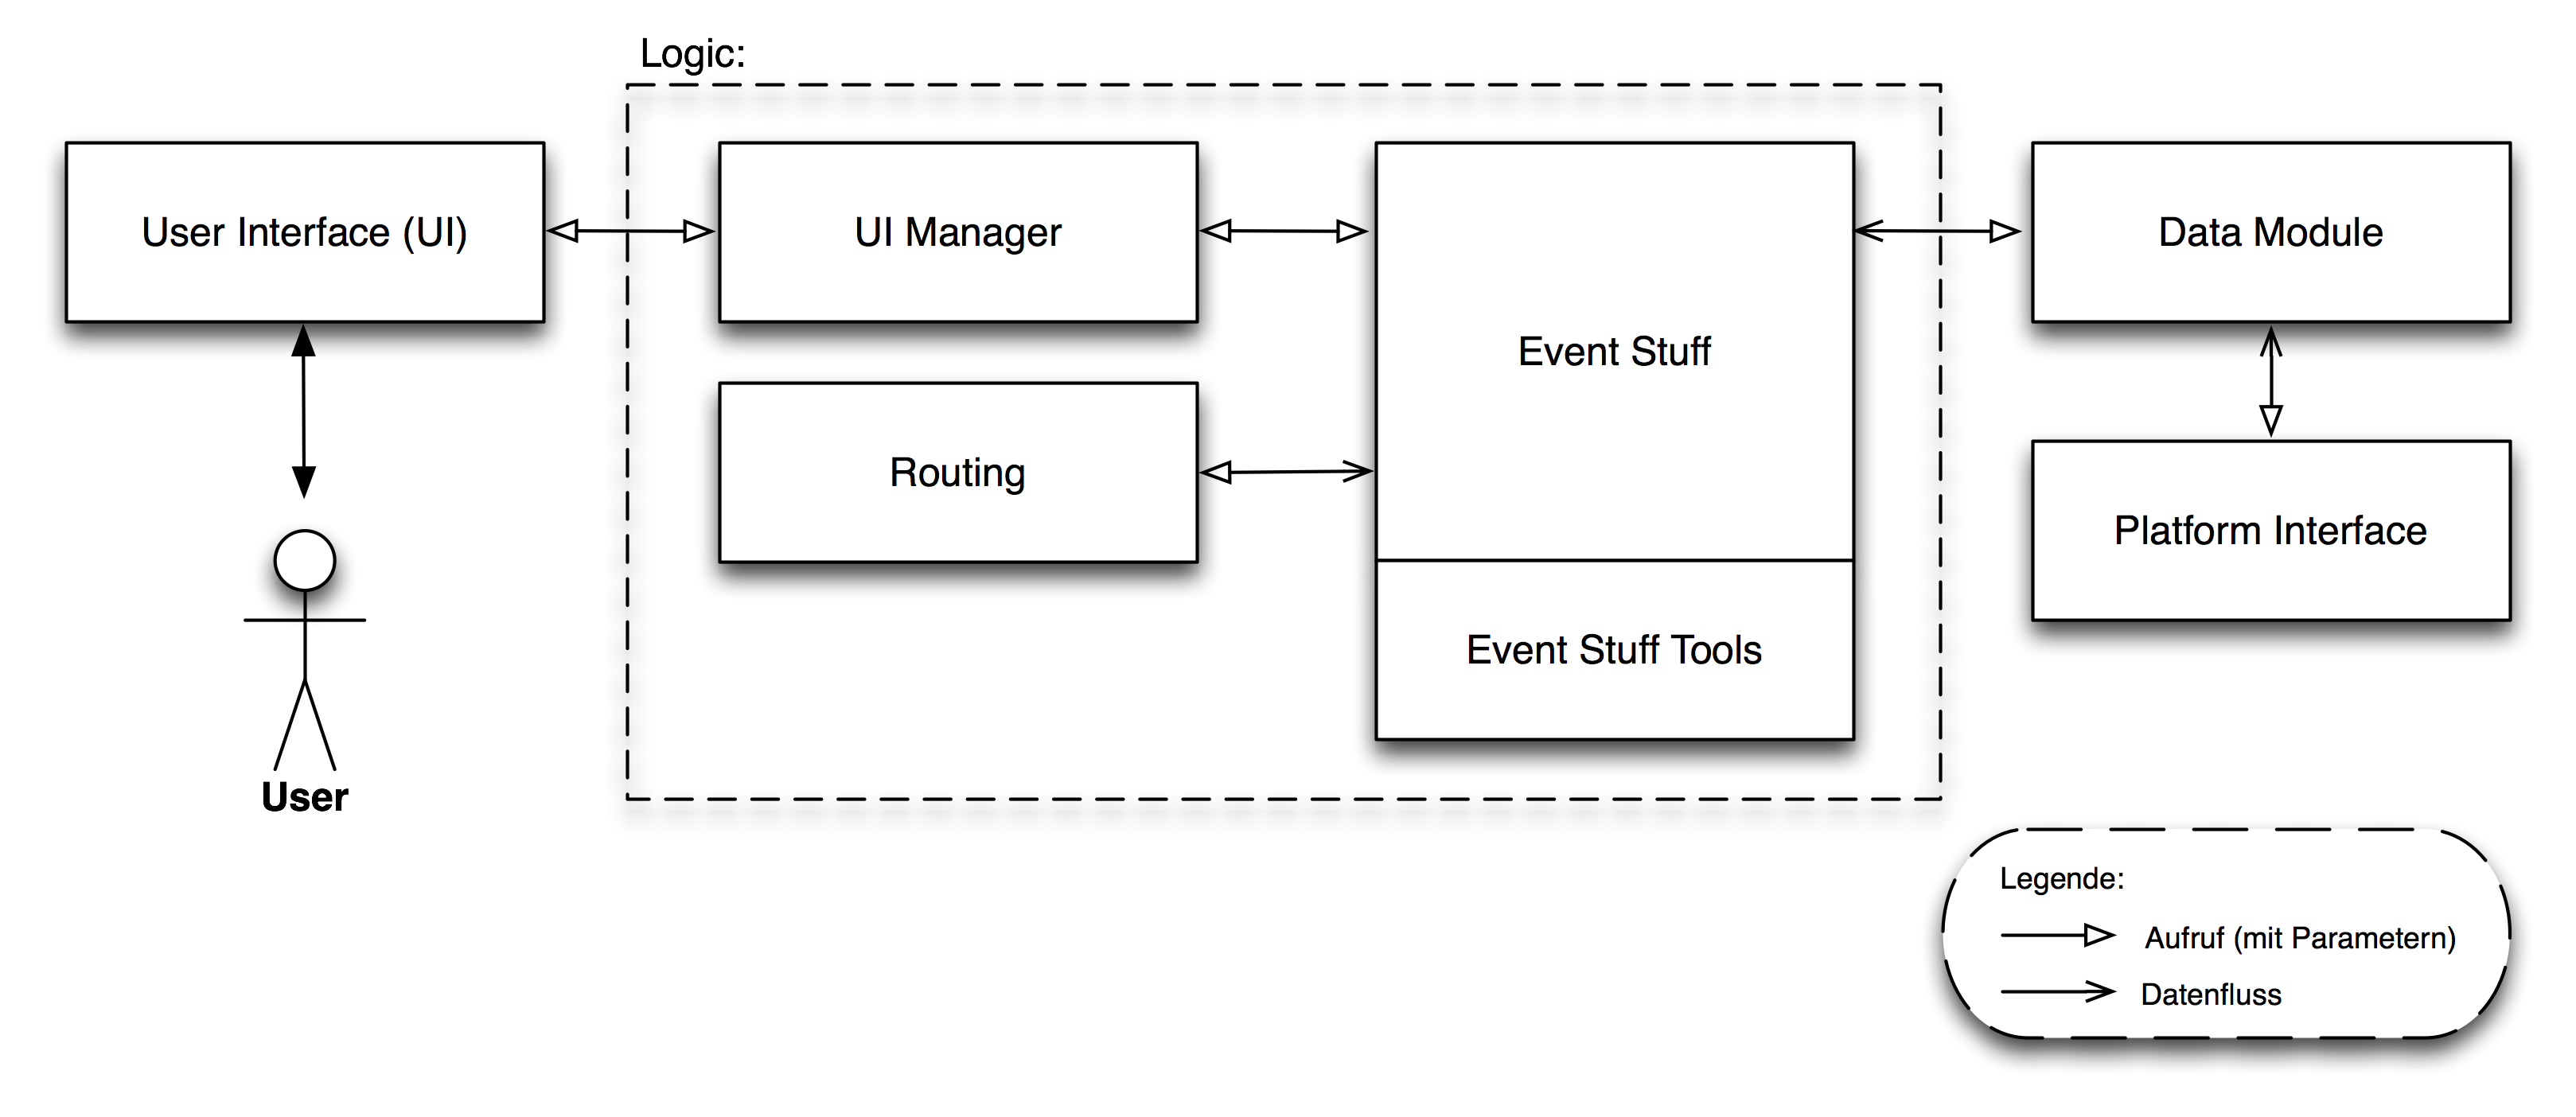
\includegraphics[width=16cm]{pics/logic.png}
\caption{Representation of the logical system elements}
\label{logic}
\end{figure}
Figure  \ref{event_stuff} shows the inner elements of the Event Stuff module. The functionality is divided into these modules:
\begin{itemize}
\item Event Warner: This module needs to run in the background it checks wether the current dayplan can be sustained, given the current position of the user in time and space. It informs the user when he hast to get going in order to meet his next appointment.
\item Plan Bauer: This module is used to create dayplans from the events and the tasks in the database.
\item Plan Optimierer: This module can optimize the current dayplan by inserting executable tasks into the dayplan at practical locations.
\item Termin Vorschkaeger: This module can be used to suggest practical locations and times for meeting between two users of this application. This can only work, when the dayplans of these two users are shared.
\item Erreichbarkeitspruefer: This module is part of the Event Stuff Tools. It can check, wether a given appointment can be reached, given a certain current point in time and space.
\item Time-Finder and Time-Filler: These are helper modules that can suggest a place and a time for a certain task to become an event of a certain deyplan. 
\end{itemize}
\begin{figure}[h!]
\centering
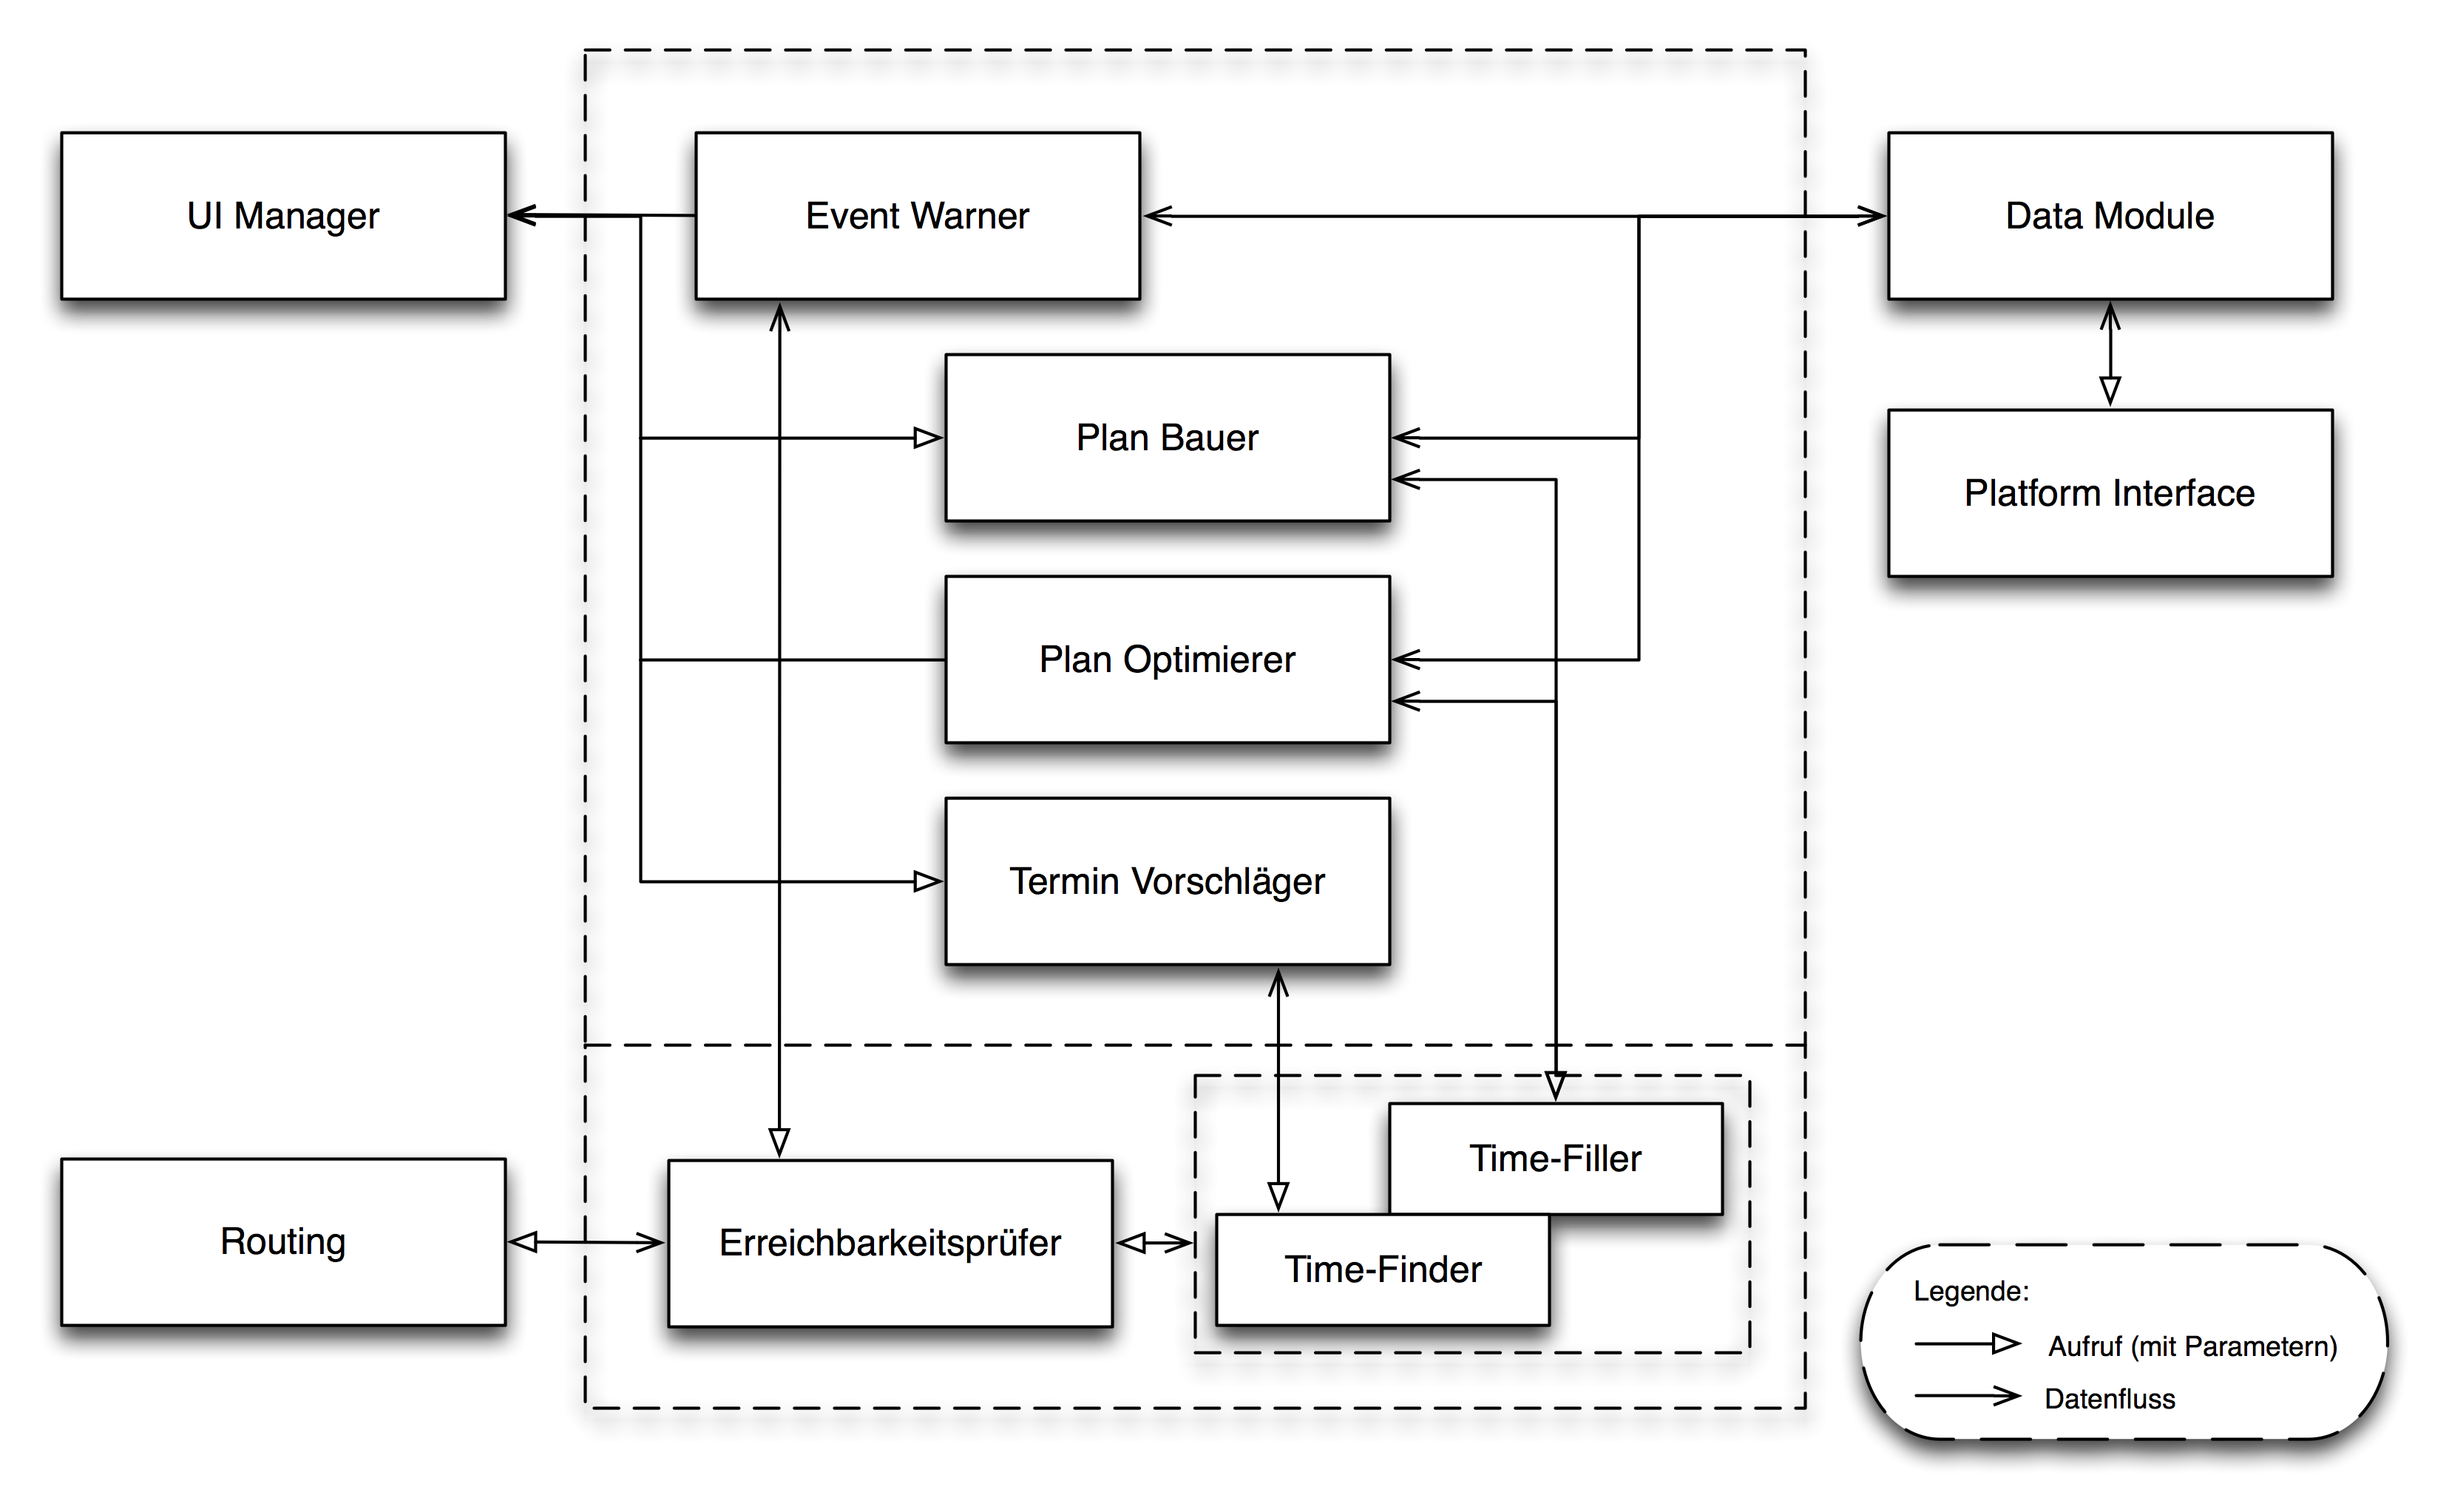
\includegraphics[width=16cm]{pics/event_stuff.png}
\caption{Components of the Appointment/Task optimization and verification engine}
\label{event_stuff}
\end{figure}

%\begin{figure}[h!]
%\centering
%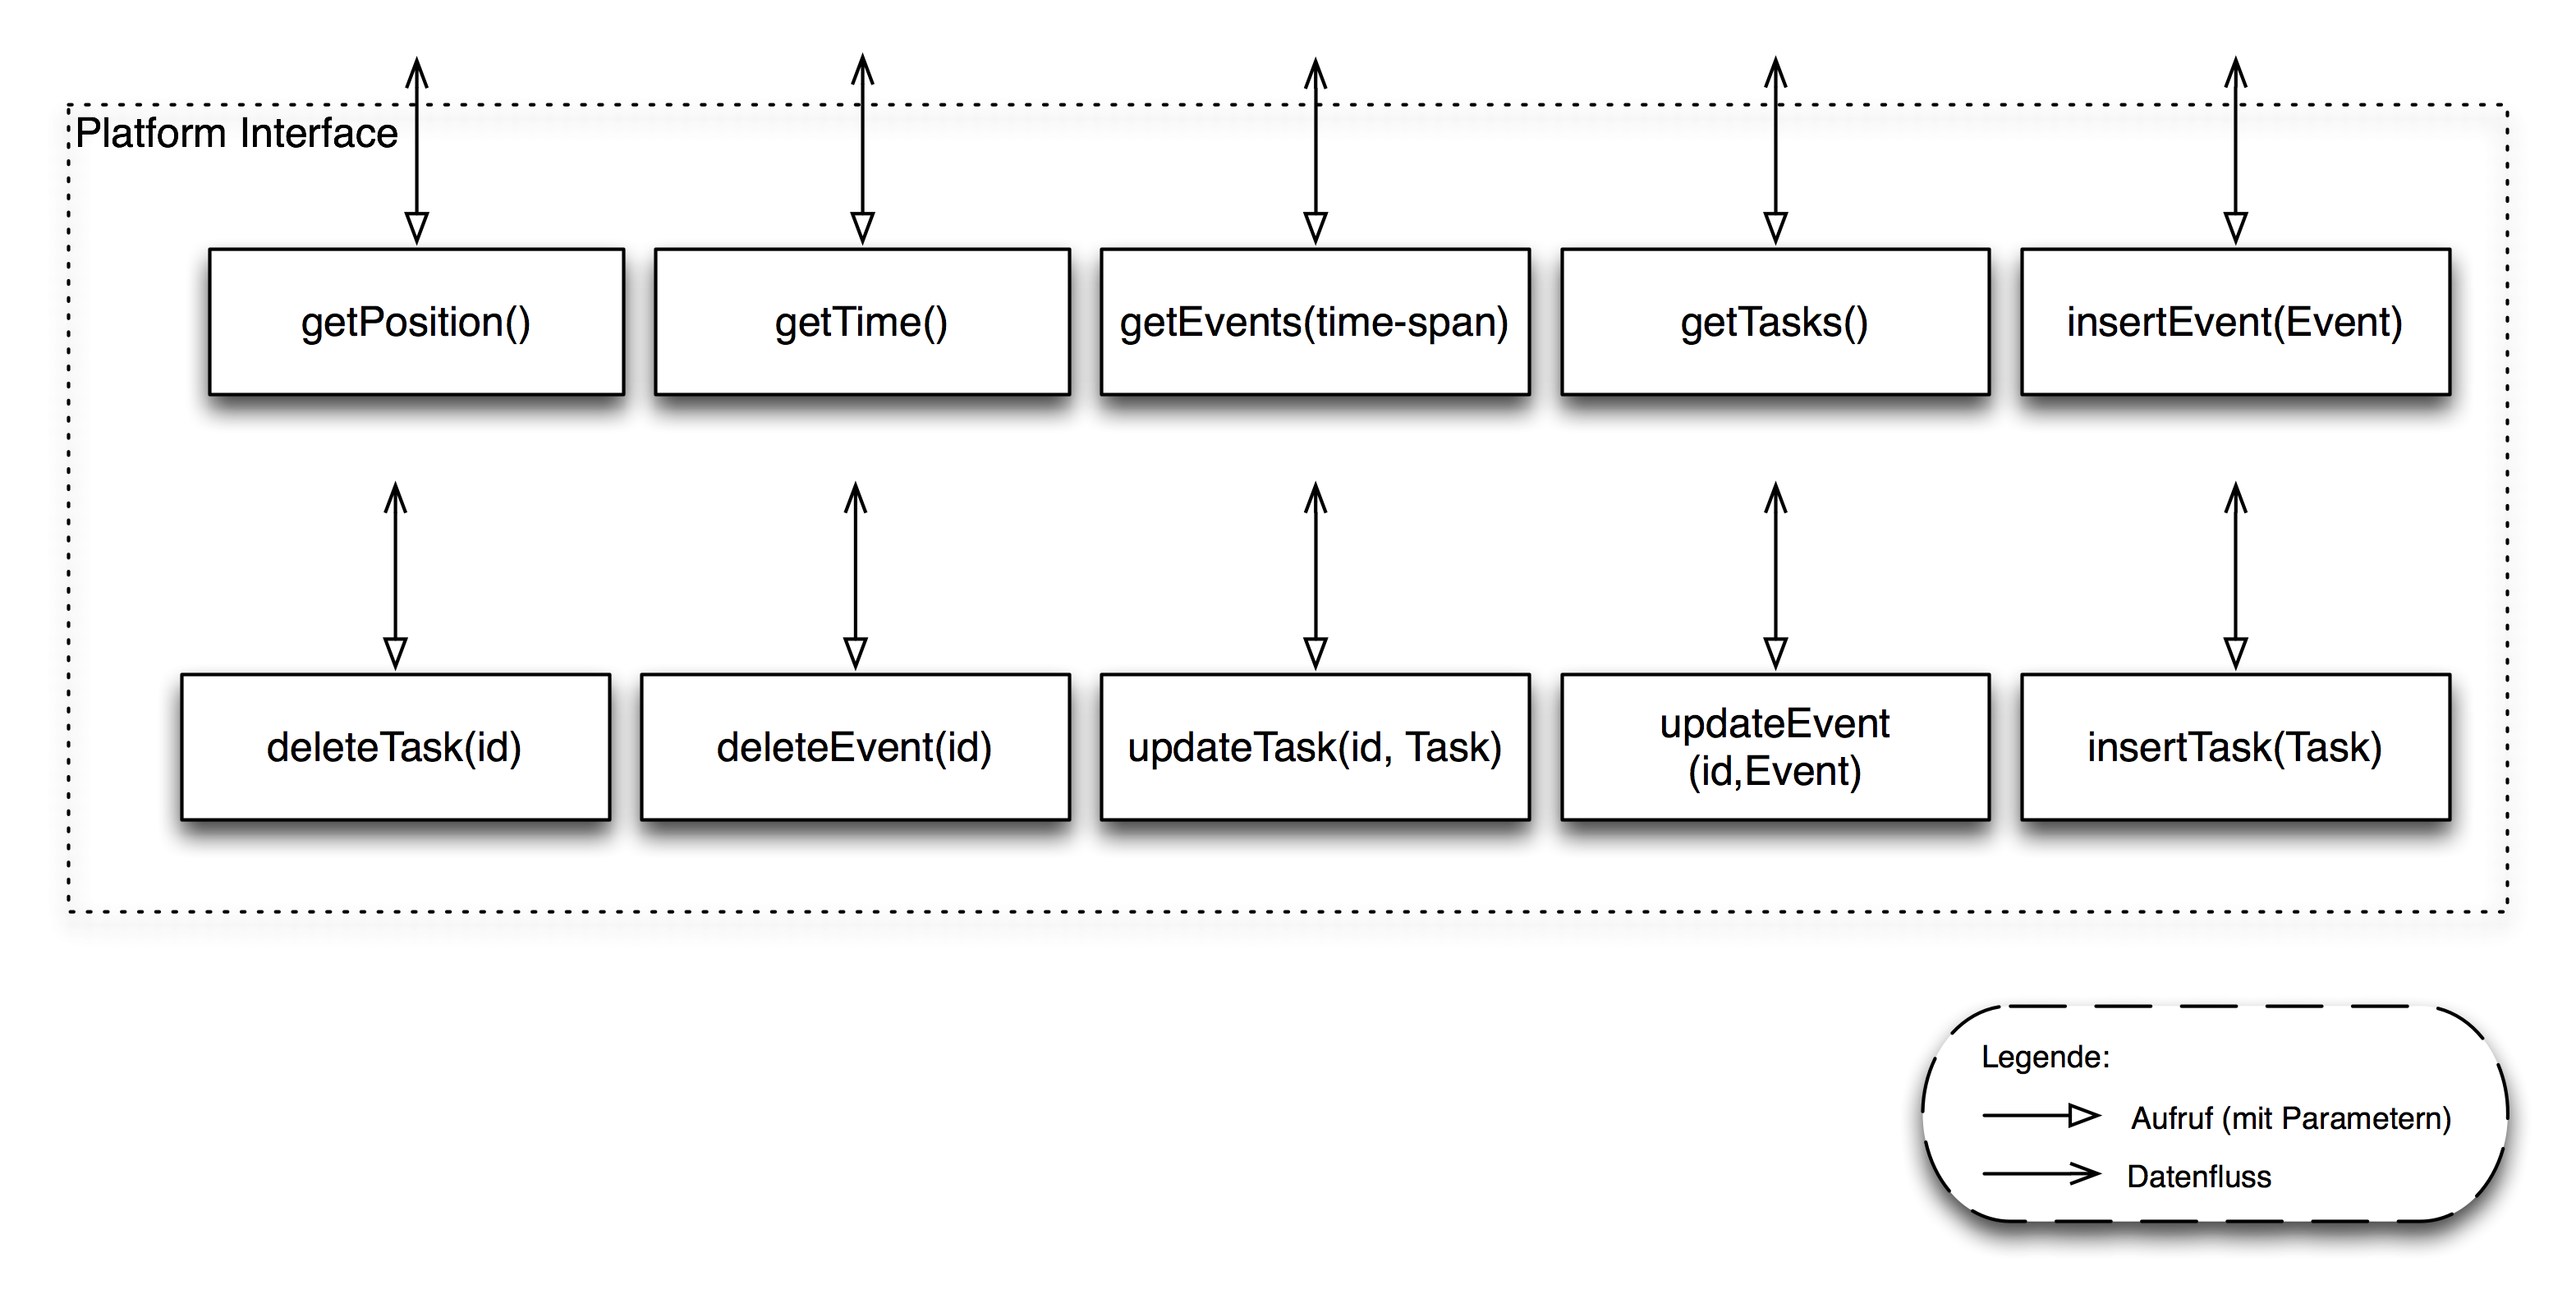
\includegraphics[width=16cm]{pics/data_module.png}
%\caption{Highlevel interface for data storage and system interaction}
%\label{gantt1}
%\end{figure}
	
%project-plan and dev. process
\chapter{Project plan and development process} % (fold)
\label{chp:project_plan}
\section{Initial project plan}

TODO: write a few sentences to describe the GANTT diagram 

\begin{figure}[h!]
\centering
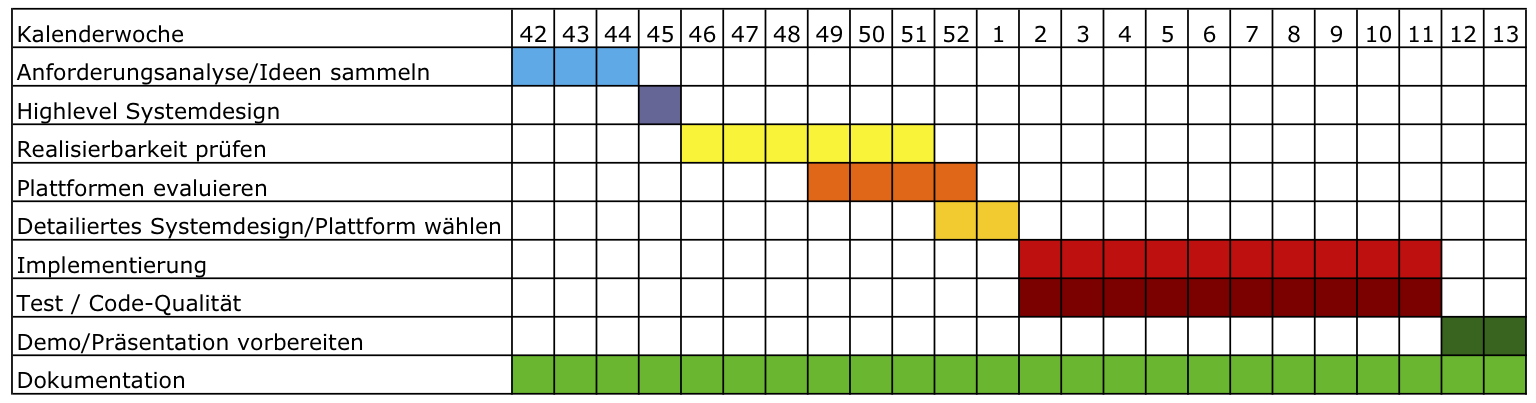
\includegraphics[width=16cm]{pics/gantt2.png}
\caption{Gantt diagram of the initial project plan (planing at project start)}
\label{gantt1}
\end{figure}

\section{Refined project plan}

TODO: insert second GANTT-diagram

TODO: extend task-list, introduce the list as milestones for second GANTT-diagram



\begin{itemize}
\item longer platform evaluation phase
\item added technology scouting phase for selected platform
\item add milestones in implementation phase
\end{itemize}
At the beginning of calendar week 7 it became obvious, that the number of open ToDos and the amount of time left until the project end after calendar week 13 required a more success-oriented development methodology.\\
For this purpose the development block (red in GANTT diagram) needs to be divided into smaller tasks or milestones, both for already completed work and for future tasks.\\

Up to this point, we were able to fulfill the following tasks:
\begin{itemize}
\item gather system requirements
\item define clean abstract system structur
\item choose appropriate OS and platform for the project
\item derive a OS specific system structure
\item install and get used to Android SDK
\item port Traveling Salesman routing engine to Android
\item solve biggest performance issues with routing engine
\item reverse-engineer the non-public Android calendar interface
\item finalize routing interface and implementation for Android
\item finalize calendar API
\item build system integration framework for Android OS, specifically  location and time triggered background tasks and user interaction
\item merge system parts into one unified application
\end{itemize}

 For the remaining 6 weeks of the project the following ToDos are left:
 \begin{itemize}
\item Determine performance of routing engine, identify bottlenecks and problems for future fixing
\item implement GUI for the task ''Generate and Manage Tasks''
\item implement GUI for the task ''Build and Manage day-plan''
\item implement background task ''optimize day-plan''
\item implement background task ''check day-plan for reachability of appointments''
\item write test-cases for the most important system parts (specifically the parts that could be reused in future projects)
\end{itemize}



	\section{Development process} % (fold)
	\label{chp:dev process}
	TODO: describe development process: iterative waterfall model with prototyping, why we chose this process, what tools we use (git) 


	
%technological evaluation
\chapter{Technology evaluation} % (fold)

	%choice of mobile platform
	\section{Platform Choice} % (fold)
	\label{chp:platform_choice}

	\subsection{Introduction} % (fold)
	\label{sec:platform_introduction}
	The usage of a mobile device is implied by the nature of the planed software project. Also the wide availability of  smart phones that come with all the hardware components we need makes it obvious that mobile phones are clearly the platform of choice. At the moment (Jan. 2010) there are three dominant operating systems for mobile phones that have to be considered for the present use case: Windows Mobile, iPhoneOS and Android. These platforms have to be evaluated in order to choose the one best suitable for our purpose.   

	\subsection{iPhone OS} % (fold)
	\label{sec:iphone}
	The iPhone is a very interesting device for mobile applications,
since it has a very modern and intuitive interface. However due
to some limitations in the iPhone OS, it is not suitable for
mobile task routing and planning.

The main limitation of the iPhone OS is the fact that it does
not allow applications to run in the background. This was a
design decision to increase battery life. This is a big problem,
since the main functionalities of the application rely on the fact
that it is always running. For example, if the application isn't
running all the time, it is not possible to warn the user about
several situations in which he needs to act to fulfill his schedule.

In the iPhone OS there are two solutions possible to circumvent this
limitation. The first one would be to have the application running all
the time, which is both impracticle and would mean that nothing else
can be done with the device during that. The second solution, which was
integrated in the newest major release of the iPhone OS, is a
notification system, which makes it possible to push messages,
notification sounds and application badges onto the device. This
however would mean, that the routing engine needs to be implemented
on a server or other external device. Then we could get position updates
from the iPhone, calculate if there was anything to be done and
notify the user accordingly. However such a scenario would impose
more threats and problems on personal privacy and is therefore not
wanted. Additionally it is not completely sure, that the position data
of the device, used for the ``Find my iPhone'' functionality, for
example, is publicly available for developers.

That is why the iPhone is not suitable as a platform.


	\subsection{Android} % (fold)
	\label{sec:android_plattform_choice}
	TODO: describe why android is the most suitable paltform:

- inexpensive devices
- open architecture: (background-tasks)
- big momentum: large dev. community, adapted by nearly every phone manufacturer
- high level language development, infrastructure for app distribution

	\subsection{Windows Mobile} % (fold)
	\label{sec:win_mobile}
	Although Windows mobile is widely used in current smart-phones, it is not the right choice for this project. For an application like Kangaroo to be accepted by potential users, it has to be easy and fun to use. With the rather clunky UI of Windows mobile (prior to version 7) a big number of custom UI elements would have been necessary to create an easily usable and ''cool'' application. The fact that none of the developers has any recent .NET experience further increases the expected time of development. Furthermore the market-share of Windows mobile is constantly shrinking, and at the time of the decision (January 2010) it remains to be seen how it can compete. 

	\subsection{Other OS} % (fold)
	\label{sec:other_os}
	There are a number of other mobile operating systems, which were not
investigated further as a development platform, namely WebOS, Blackberry OS, SymbianOS and Maemo.
The Main reasons for this are:
\begin{itemize}
  \item A small significance for the mobile market
  \item A complicated or not yet matured development process
  \item UI- or system- limitations that prevent a proper implementation of Kangaroo
\end{itemize}


	
	%routing
	\section{Routing} % (fold)
	\label{sec:android_routing}
	One essential feature of our application is its capability to not only consider calendar items for itself but to put them in their geographical context and to account for local traffic facilities. This implies the need for a set of data representing these facilites and an engine to operate on the data.\newline

From a very abstract and general perspective, this set of data can be divided into two categories, namely a dynamic and a static one. As static, in these terms, one should label all facilities which do not depend on any schedule and may in principle by used at any time (for example streets and highways). Dynamic facilities are the ones, that have a more or less fixed schedule constraining their usage (for example tramways and public bus service).\newline

In this project we will only consider static facilities, since also accounting for dynamic ones requires routing algorithms that go far beyond standard algorithms resulting in a more complex application structure and a much more complex routing engine. Besides this aspect, it is a big issue to gather scheduling data about dynamic traffic facilities as there would be a number of carriers with different interfaces to include. However, the user might notably benefit from the abolishment of this restriction. It might be part of future work to include this feature.\newline
 
As potential sources for static traffic facility data, one finds basically two options

\begin{itemize}
 
	\item \textbf{Google Maps}
	
		Google Maps is an online navigation and routing service. Its map material has high quality but in some areas lacks actuality. Its main drawback may anyway be found in the absence of a free simple-to-use offline interface. 
	
	\item \textbf{Openstreetmap}
	
		Openstreetmap is a free and open database for a world wide map. Everyone is free to add, change and remove map items. Consequently its map material varies over a hugh scale in quality, density and actuality. It can be used online and offline by downloading an Openstreetmap XML file of a rectangular map area. This file contains every map item of this area.
  
\end{itemize} 

Besides the two options given above there are of course lots of other providers, but either not free of charge or not very popular. Consequently, Openstreetmap seems to be the one to choose for our project. The following will briefly outline its data scheme.\newline

\subsubsection{Data scheme of Openstreetmap}

Openstreetmap uses three main entities to map traffic facilities and geographical characteristics:

\begin{itemize}

	\item \textbf{Nodes}
	
		Nodes are the fundamental elements setting up model points for direct use or as a basis for superior map elements. A node imperatively has a unique ID and values for latitude and longitude, but can have optional parameters provided as tags with key-value-pairs. Adding tags to a node is the way to define, for example, Points Of Interest (POI).
		
	\item \textbf{Ways}
	
		Ways are made up of an ordered list of nodes which span the way in the given order. Just like a node, a way must have a unique\footnote{unique with respect to other ways; there still might be a node with the same ID} ID and may have optional tags.\newline
		As a way can either be closed\footnote{first and last nodes are the same} or open and can have tags to specifiy parameters, it can be used to map streets, highways, roundabouts, buildings or even administrative areas.	
		
	\item \textbf{Relations}
	
		Realtions provide a simple way to group other map elements. This feature will not be used.
	
\end{itemize}

	
	\subsection{Routing engines}
	\label{sub:routing_engines}
	In our project's scope, the routing engine is ought to be used and thus its output is required to give answer to the following two questions:

\begin{enumerate}

	\item How long does it (approximately) take to follow the shortest path between two locations?
	
		To give a good answer to this question, one has not only to specify two locations as starting point and destination of the route, but also a vehicle that will be used to travel this route, since its choice might influence\footnote{think of oneways which normally are free to be used in both directions when for example riding a bicycle} the route. In addition to this, remember we are mainly interested in the \emph{time} needed to travel the route, not its \emph{distance}. For this, in a first step we have to combine the maximum speed of the vehicle with the distance of the route. As a secound step, one should also consider local speed limitations, which effectively influence the vehicle's maximum speed on a certain part of the route.
	
	\item Where, looking from a specfic location, is (are) the next Point(s) Of Interest providing a specific type of service?
	
		Finding a statisfying answer to that question is in principle very easy. One has to scan the local area around the given center for facilities that match the criteria and give a list of the nearest ones.

\end{enumerate}

Having defined the information we are aiming for when triggering an operation of the routing engine, the following gives a brief overview of already existing open source routing engines that may be used in our project:

\begin{enumerate}

	\item \textbf{Gosmore}
	
		Gosmore is a routing and navigation software for mobile devices. It consequently also consists of a very efficient routing engine to operate on data coming originally from Openstreetmap, but which is reorganized and compressed in a very smart way in advance. For this, data is ordered in a way that tries to minimize the probablity of a cache-miss and the number of comparisons needed when searching the local map for special map elements.
		Gosmore is based on C/C++, very compact and makes extensive use of pointers and indirect memory access. Documentation of its source code is poor and thus it is not easy to comprehend and retrace its code.
	
	\item \textbf{OSMAndroid}
	
		OSMAndroid is a map viewer and routing engine for Android using precompiled Openstreetmap data. It uses a special OSMAndroidConverter to parse the bulky Openstreetmap XML file and to compress it to an extremely small 	proprietary data structure, maintaining only map elements needed for routing. Its very slight data model results in little and fast data access operations and very efficient routing operations.
		OSMAndroid's source code has rare comments and follows a sometimes confusing design pattern, but is because of its compactness understandable with not to much effort.
	
	\item \textbf{Traveling Salesman (TSM)}
	
		Traveling Salesman is a Java based open source navigation and routing framework using Openstreetmap data as its input\footnote{actually it is using Osmosis as an interface to Openstreetmap data, which is a java application for processing Openstreetmap data}. It has a consistent modular architecture and allows to assemble a specific navigation software nearly ''just-as-you-like''. Traveling Salesman comes with ready-to-use implementations for every module. These modules are by default designed to keep every map element and not to filter irrelevant\footnote{irrelevant in the sense that the result of any operation that may be performed does not depend on the element's presence or absence} ones. This results in a maximum generality at the cost of performance and memory space.
		Traveling Salesman is up to now still in beta stage.

\end{enumerate}

Since the target platform is a mobile one and resources will be limited, handling of available device resources is a crucial issue in the decision for a routing engine. Nevertheless it is not the only thing to think of in this context. In addition to the output requirements mentioned at the beginning of this chapter, there are other issues to account for. Some of them are for example the portability to our target platform and the flexibility for future adaptions and extensions.\newline

When trying to assign priorities to these aspects just mentioned before, one will be faced with the question whether to aim for a maximum of flexibility or for a maximum of performance, since these two features are contradictory in many ways. Traveling Salesman is situated near the end of the scale where focus is set on a maximum of flexibility, while Gosmore and OSMAndroid can be found near the other end. Balancing these priorities was dynamically done during technology scouting and therefore the next chapter will give considerations and results on this aspect in greater detail.\newline

Anyhow, as an integral part of the abstraction of the application's structure, the routing interface is designed in a way, that makes it independent of the decision for any routing engine, even if its design was influenced by it. This means, that although a final decision had to be made within the scope of our project, there is still the chance to choose another engine as part of future work.\newline

\subsubsection{Technology scouting - general part}

This section will give an overview of the general Technology Scouting process.\newline

Before focusing on a single routing engine, we analyzed the given options of routing engines with respect to our definitions. Unfortunately when doing the technology scouting, we did not know about the OSMAndroid routing engine and thus had no chance to consider it in the decision for a routing engine. Although its analysis has been done when a final decision already had been made and the technology scouting phase had been finished, the reasons for us not to change this decision afterwards will be given in this chapter.\newline

With the two options given at the beginning of the technology scouting phase, Gosmore and Traveling Salesman, the Traveling Salesman project had the considerable advantage of being based on Java, in contrast to Gosmore, which is effectively a C/C++ library. This fact gave rise to put first focus on Traveling Salesman to identify its drawbacks and opportunities.\newline

As our analysis revealed that Traveling Salesman is the most promising option\footnote{remember the only alternative at that time was Gosmore}, a discussion of this analysis will be given in a later chapter in greater detail. At this point, we will give a rough overview of the analysis of Gosmore, Traveling Salesman and OSMAndroid. In Addition to these three we will give a summary of considerations towards a proprietary development at the best combining advantages and opportunities of existing projects and excluding performance bottlenecks.\newline

\begin{itemize}

	\item \textbf{Gosmore}	
	
		TODO: explain why not Gosmore
	
	\item \textbf{Traveling Salesman (TSM)}
	
		First integration of Traveling Salesman's library into an Android project was rather simple, just as one would expect. It was integrated into a first application which was designed to use TSM to read an Openstreetmap XML file stored on the SD card of the mobile device and to output the file's summarized content. Compiling and running this application was possible without any errors but revealed three initial problems:
		
		\begin{itemize}
		
			\item Traveling Salesman uses a proprietary \texttt{FileLoader} class to read the Openstreetmap XML file and to initialize a  \texttt{MemoryDataSet} object holding all data from the XML file. This \texttt{FileLoader} in turn uses the java built-in  \texttt{SAXParser}\footnote{ \texttt{javax.xml.parsers.SAXParser}} class and an extension of the  \texttt{DefaultHandler}\footnote{\texttt{org.xml.sax.helpers.DefaultHandler}} class which seem to be implemented slightly different in Android's java library. A permutation in the parameters of the method  \texttt{startElement(...)} yielded a complete discapability of reading the XML file, but could be overcome by re-permutating its parameters.
			
			\item After having fixed the problem given in the previous clause, Traveling Salesman did its first job on both the emulator and a physical mobile device. With minor additions to our application, we were able to perfom a \texttt{getNearestNode(...)} query on a tiny data set, showing that we will get into big trouble concerning performance, if no adaptions were applied. However, we were able to show that improving Traveling Salesman's performance in a way satisfying our requirements is in principle possible and an issue one will be able to deal with (chapter \ref{sec:techscout_routing_specific} will give details).	

			\item memory usage	
		
		\end{itemize}

	\item \textbf{proprietary development}

		The possibility to use the given routing engines only as a source of inspiration and to start a proprietary development began to cross our minds, when ideas of how to design a routing engine became clear. Deliberation of combining a slight and efficient data storage system (like Gosmore is using), a reduced routing graph to operate on and java based source code (like Traveling Salesman has) occupied our minds. This thoughts were triggered by becoming aware of the fact that Traveling Salesman is in principle much more than we need and Gosmore in turn would need too much manipulations to be compatible with the Android system.

	\item \textbf{OSMAndroid}

		TODO: explain why not OSMAndroid	

\end{itemize}

Eventually we decided to base the routing engine on the Traveling Salesman project, maintaining compatibility to its modular architecture. This decision was forced by the following reasons

\begin{itemize}
	\item Java based source code
	
		Traveling Salesman is completely based on Java and does not use any external libraries. Its precompiled project library can easily be integrated in the Android environment and Android projects following the standard design approach and thus requiring zero investment in any abnormality with respect to this standard.
	
	\item adaptions and extensions may be implemented without touching its inner structure
	
		Traveling Salesman's modular architecture supports easy exchange of any of its components. Given the imperative need of an adapted data storage management system to improve utilization of resources, we could easily come up with a re-design of this component without the need of adapting other components. The same applies to modifications of both the routing algorithm and its routing metric which can each be modified independently of the other.
	
	\item maximum generality and flexibilty, exchangeable components
	
		Keeping compatibility to Traveling Salesman's modular architecture will offer the chance for easy maintenance or even upgrades. One may consequently benefit from future modifications made to the original Traveling Salesman project.
	
	\item performance improvements
	
		Early progress made with improving its performance gave rise to the assumption, that the advantages given in the clauses before will doubtlessly outweight the loss of performance and advantages provided by other solutions.
		
	\item "flexibility before performance"
	
		Last but not least, ...
	
\end{itemize}


The following chapter will give a more detailed introduction in the structure of Traveling Salesman.

\subsubsection{Traveling Salesman}

As already mentioned, Traveling Salesman is designed following a modular architecture. Every essential or optional type of module is defined by a java interface with basic methods to provide its desired functionality. The most important ones in our project are

\begin{itemize}

	\item Interface \texttt{IDataSet}
	
		\texttt{IDataSet} provides methods to store and receive Openstreetmap map elements. Identification of elements to receive can either be done by unique Openstreetmap ID or by parameters to search for. This, for example, may be the name of the element or simply its distance to a specific point, that has to fall below a cetain value.\newline
		 In dependence of its implementation, data storage is done in memory (\texttt{MemoryDataSet}), on disc or in a database.
	
	\item Interface \texttt{IRouter}

		\texttt{IRouter} is the interface which has to be implemented by any routing class. Its primary task is triggered by calling the \texttt{route(...)} method, which performs routing between a point to start from an one or more destination points. One has to pass an \texttt{IDataSet} object specifying routing resources, when calling \texttt{route(...)}. The router is to return a \texttt{Route} object containing detailed information about the path.
	
	\item Interface \texttt{IRoutingMetric}
	
		As to give the router a  measure of routing costs, one has to define a class implementing the \texttt{IRoutingMetric} interface, which allows the router to query routing costs of particular routing steps.\newline
		The default implementation (\texttt{ShortestRouteMetric}) simply measures distance between start and end of a routing step. One might feel uncomfortable with this, because it does not privilege any type of street and hence the shortest route is probably not the fastest one. However, this can be overcome with a re-implementation of a routing metric.
	
\end{itemize}

To represent Openstreetmap map elements (nodes, ways and relations), Traveling Salesman uses classes provided by Osmosis, which can be considered as a Java based framework for processing of Openstreetmap data. Osmosis employs classes named \texttt{Node}, \texttt{Way} and \texttt{Relation} to represent Openstreetmap map elements accordingly. 

\subsubsection{Technology scouting - specific part}
\label{sec:techscout_routing_specific}

This section will give an overview over the Traveling Salesman specific Technology Scouting process.\newline

- changes applied to the XML parser

- test system (mainly map file) used to make first progress with performance

[...]


	\subsection{Traveling Salesman}
	\label{sub:routing_tsm}
	The following chapter will give a more detailed introduction in the structure of Traveling Salesman.\newline

As already mentioned, Traveling Salesman is designed following a modular architecture. Every essential or optional type of module is defined by a java interface with basic methods to provide its desired functionality. The most important ones in our project are

\begin{itemize}

	\item Interface \texttt{IDataSet}
	
		\texttt{IDataSet} provides methods to store and receive Openstreetmap map elements. Identification of elements to receive can either be done by unique Openstreetmap ID or by parameters to search for. This, for example, may be the name of the element or simply its distance to a specific point, that has to fall below a cetain value.\newline
		 In dependence of its implementation, data storage is done in memory (\texttt{MemoryDataSet}), on disc or in a database.
	
	\item Interface \texttt{IRouter}

		\texttt{IRouter} is the interface which has to be implemented by any routing class. Its primary task is triggered by calling the \texttt{route(...)} method, which performs routing between a point to start from an one or more destination points. One has to pass an \texttt{IDataSet} object specifying routing resources, when calling \texttt{route(...)}. The router is to return a \texttt{Route} object containing detailed information about the path.
	
	\item Interface \texttt{IRoutingMetric}
	
		As to give the router a  measure of routing costs, one has to define a class implementing the \texttt{IRoutingMetric} interface, which allows the router to query routing costs of particular routing steps.\newline
		The default implementation (\texttt{ShortestRouteMetric}) simply measures distance between start and end of a routing step. One might feel uncomfortable with this, because it does not privilege any type of street and hence the shortest route is probably not the fastest one. However, this can be overcome with a re-implementation of a routing metric.
	
\end{itemize}

To represent Openstreetmap map elements (nodes, ways and relations), Traveling Salesman uses classes provided by Osmosis, which can be considered as a Java based framework for processing of Openstreetmap data. Osmosis employs classes named \texttt{Node}, \texttt{Way} and \texttt{Relation} to represent Openstreetmap map elements accordingly. 
	
%kangaroo for android

\chapter{Developement for Android} % (fold)
\label{chp:android}
%Kangaroo was developed as a team project at the Albert Ludwig University of
Freiburg. The goal was to develop an application which knows all events and
tasks data of a user. Based on this information, the best route to attend all
events and complete as many tasks as possible, is computed. In this document,
all information which was created during the development is collected.

Chapter 2 describes the requirements as defined by the Lehrstuhl, as well as the
resulting development goals and the abstract system structure that was designed
to fulfill these requirements.

Chapter 3 contains information about project planning and the development
process. This means the initial and refined project plan as well as the
description of the development process.

The process of evaluating suitable platforms is described in chapter 4. The main
focus here lies on the three mobile Operating Systems iPhone OS, Android and
Windows Mobile. Others are also described briefly. Additionally the decision
which routing engine to use is described in this chapter, too.

The actual development process is the focus of chapter 5. Here the platform
specifics, which impact the system design, are explained. Furthermore the main
parts of the application, as well as some important implementation details and
caveats are discussed.

The last chapter then provides a summary of the work with some reflections on
the completed work as well as an outlook, how to use this for future
development.


	%system specific software design
	\section{Platform Specific System Design} % (fold)
	\label{sec:android_desing}
	Based on the abstract system structure in presented in chapter \ref{chp:structure} a platform specific software structure needs to be defined for the Android OS platform.This structure is shown in figure \ref{android_structure}. It respects Android specific constructs, patterns and object-types.
\begin{figure}[h!]
\centering
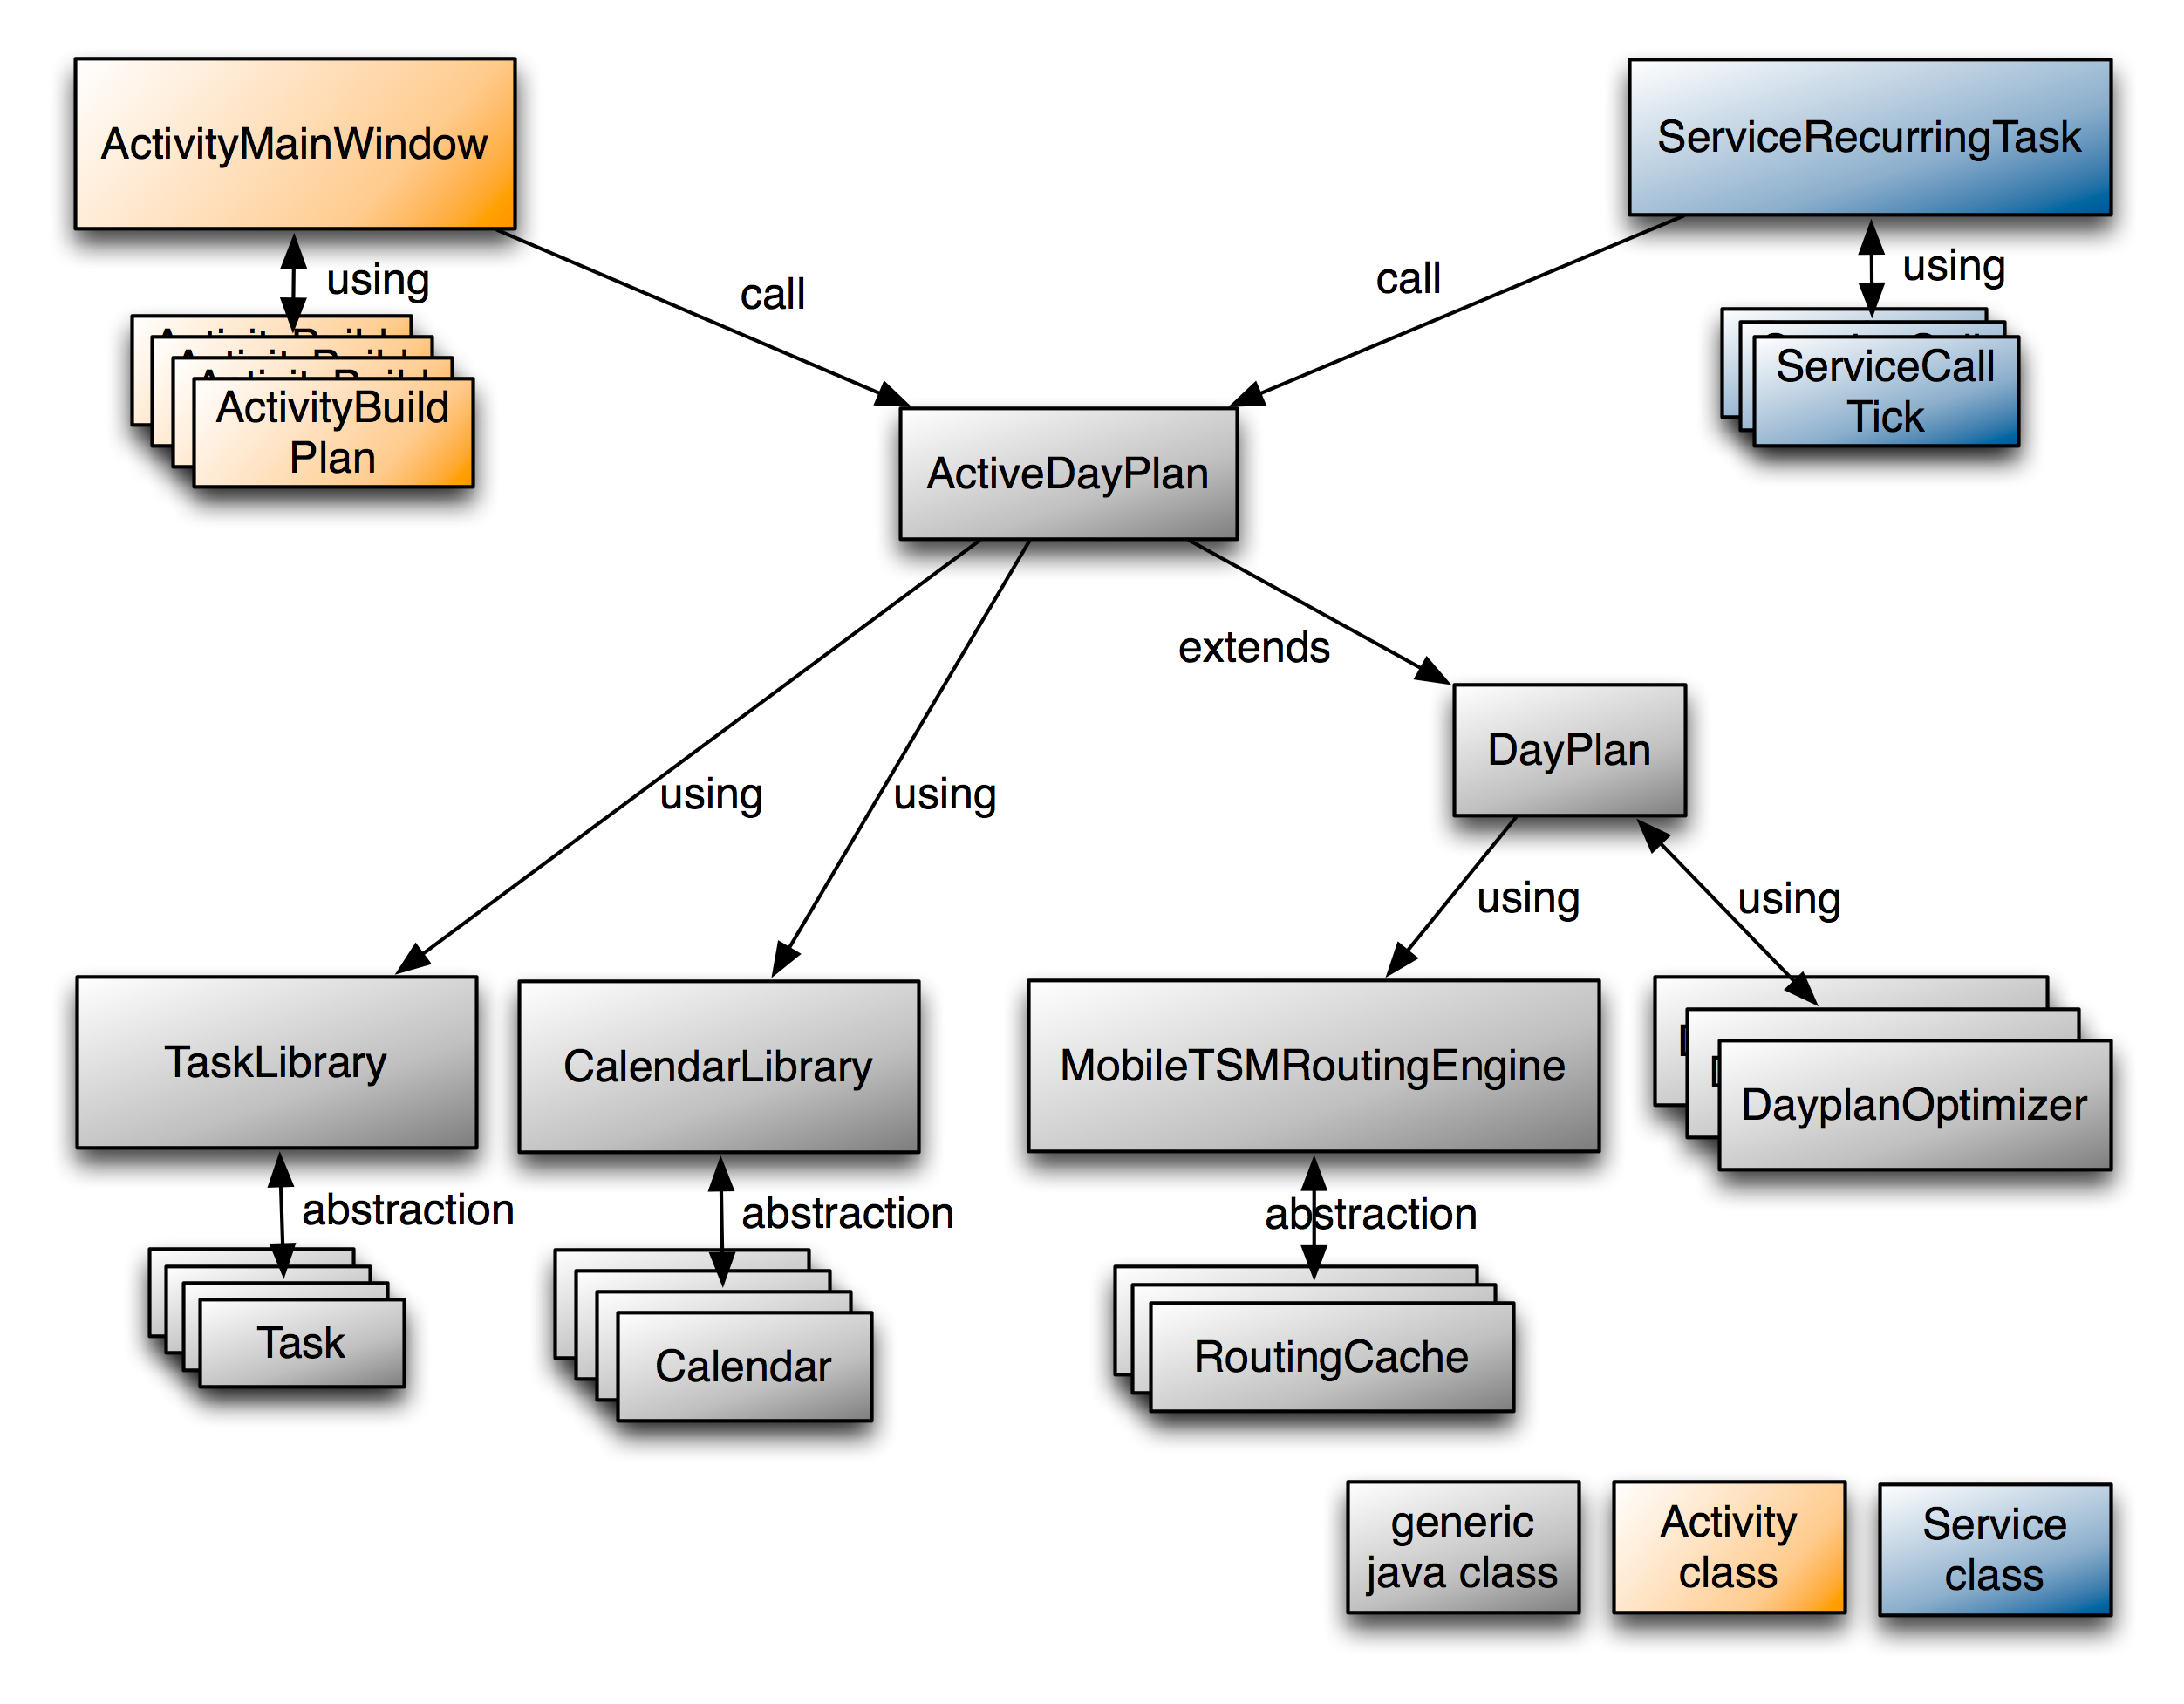
\includegraphics[width=14cm]{pics/android_structure.png}
\caption{Platform specific software structure for Android OS}
\label{android_structure}
\end{figure}
The classes marked in orange extend the platform specific Activity-class. In Android OS, Activities are used to build the graphical user interface (GUI). The class ActivityMainWindow contains a tabbing element, the other Activities are wrapped in the individual tabs. 

The blue classes extend the Service-class. Android OS uses Services to execute computations that are independent of the user interface. The background task that needs to be called cyclic is implemented in the ServiceRecurringTask. The other Services are helper classes that make sure the background task is called when the location of the device in time or space has changed.

All classes kept in grey are generic java classes. These system elements do not directly extend the Android platform, although some of them my use platform specific data types and methods.
  
TODO: describe the graphic\\
TODO: write why we did the design like that (briefly introduce android SW structure with services, activities etc.)
	
	%description of system parts
	\section{Description of system elements} % (fold)
	
	\subsection{User Interface} % (fold)
	\label{sec:user_interface}
	\subsubsection{Basic Interface Structure} % (fold)
\label{ssub:Basic Interface Structure}
The Android user interface is built upon an XML templating engine.
The basic interface is designed via XML templates and later on adapted
and filled with content via Java methods. Every Activity class inherits
from a basic activity class like ``TabActivity'' or ``ListActivity''.
The XML templates define a basic element of the according class also
(``TabHost'', ``ListView'').

% subsubsection Basic Interface Structure (end)

\subsubsection{Main Window} % (fold)
\label{ssub:MainWindow}

The main window is just the skeleton with the tablist, which then
contains the active window itself. The Activities are added
via Intents into the tabbar. An important point, when entering the embedded
Activities into the application's manifest file, is to add the intent filter
\begin{verbatim}
<category android:name="android.intent.category.EMBED"></category>
\end{verbatim}
also. This makes sure, that the Activity respects the boundaries of the
main window when activated.

% subsubsection Main Window (end)

\subsubsection{Dayplan} % (fold)
\label{ssub:Dayplan}
The DayPlan Activity is the basic status interface which shows the current
dayplan in a list. It also contains a context menu for manipulating events
and an application menu to reload events and invoke the optimizer. The
templating for this Activity consists of a template for the ListView and a
separate template for the single rows.

In order create the view, the list of events is fetched from the
ActiveDayPlan. After that a custom ArrayAdapter is used to populate the
single rows of the ListView.
The only slight problem is to get the correct object from the ArrayList,
when tapping a row in the Activity. Fortunately, when the onCreateContextMenu
method is called, it is passed a ContextMenuInfo object as a parameter. This
object contains an id, which is the same as the position in the original
ArrayList from which the view was populated. Therefore it can be used as an
index to identify the correct object in the list.

% subsubsection Dayplan (end)

\subsubsection{Tasklist} % (fold)
\label{ssub:Tasklist}
The Tasklist Activity displays all the available tasks. It is a two level
list view, which shows the task title in the first level and the task details
on expansion of an entry. It also contains a context menu to manipulate single
tasks and an application menu to add new tasks. The templating for this
Activity is more advanced, as there has to be a template for the ListView
itself, the first level and second level of rows.

The TaskList was slightly more difficult to implement as it is a two-level
ExpandableListView and therefore naturally more complicated. The most important
part is building the entries, as the ListAdapter expects a List of Maps of
Strings to Strings for the first level entries (the task titles) and a List
of List of Maps of Strings to Strings for the second level entries. The
constructor for the adapter (SimpleExpandableListAdapter) then takes these
data structures along with String arrays matching the keys of the passed Maps
and Int arrays containing the IDs of the elements in the respective XML
template for the first or second rows.

% subsubsection Tasklist (end)


	
	\subsection{Background tasks} % (fold)
	\label{sec:android_integration}
	In Kangaroo certain computations need to be performed in the background periodically.  Android OS provides a nice solution for this requirement with the Service class. Each class that extends Service can perform computations without the need of a foreground user interface. The only mandatory element that needs to be overwritten is the onCreate() method. This method is called when a new instance of the class is created. Once the service sleeps in memory until it is called, unless the phone runs out of RAM. in that case the object is terminated, so has no control over its lifecycle. When a service is called with the corresponding intent its onStart() method is called.\\\\
\begin{figure}[h!]
\centering
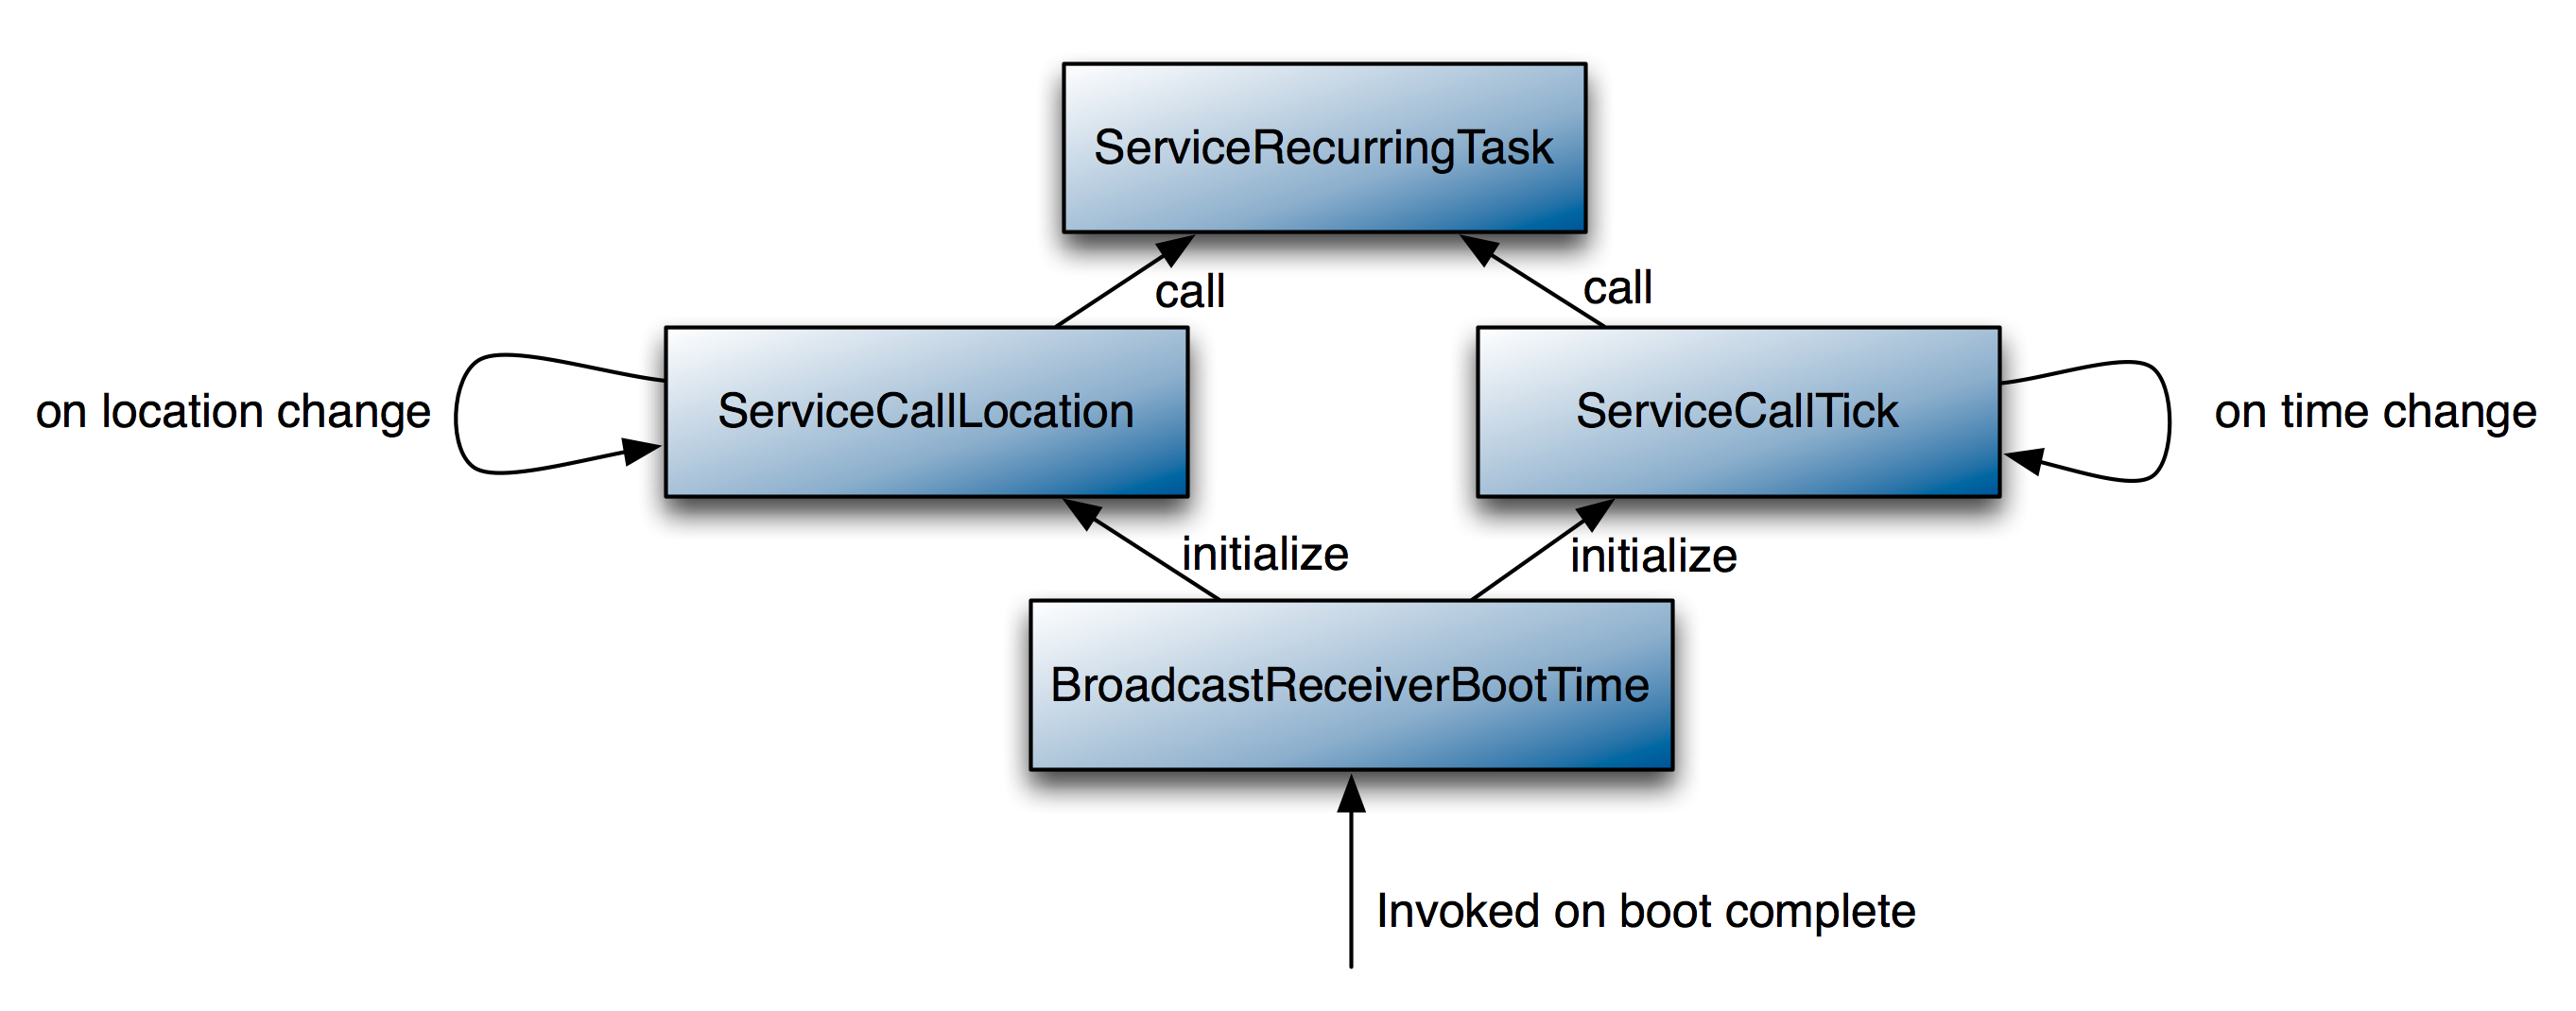
\includegraphics[width=14cm]{pics/background1.png}
\caption{Interaction of the background task classes}
\label{background1}
\end{figure}  
The services implemented in Kangaroo are located in the com.kangaroo.system package and shown in figure \ref{background1}. The BroadcastReceiverBootTime implements a BroadcastReceiver that listens to the boot-time broadcast from the OS. The receiver can be registered for a certain broadcast in the AndroidManifest.xml.
\begin{verbatim}  
  <intent-filter>	  
      <action android:name=''android.intent.action.BOOT_COMPLETED'' />
  </intent-filter>
\end{verbatim}
Once the phone has started correctly the code in the onReceive() method is executed. Here the services ServiceCallLocation and ServiceCallTick are started. ServiceCallLocation registers itself with the Android LocationManager. The service is then called every time the location of the phone has changed more than x meters. 
ServiceCallTick registers  with the AlarmManager. It is called every time a certain amount of time has passed.
Both of the services execute one task in their onStart() method: they call the ServiceRecurringTask with a corresponding intent:
 \begin{verbatim}  
Intent callIntent = new Intent(ServiceCallTick.this, ServiceRecurringTask.class);
callIntent.putExtra("isLocation", false);
startService(callIntent);
\end{verbatim}
In the ServiceRecurringTask the commands shown in figure \ref{background2} are executed.
\begin{itemize}
\item First the semaphore is checked. Since location and time updates occur independently of each other, the semaphore prevents the ServiceRecurringTask from being called multiple times simultaneously. 
\item Then a new thread is created. Since the service is executed in the main tread of the application, performing extensive calculations without a separate thread could cause the GUI to lag. 
\item Next a wake-lock on the CPU is obtained to prevent Android from putting the process to sleep. It is very important to release the wake-lock as soon as possible, since the inability of the CPU to go to a low power state drains the phone battery quickly. 
\item After that an instance of the com.kangaroo.ActiveDayPlan is acquired and the methods to check consistency and reachability of the day plan are called. If the plan is not consistent or a event can not be reached in time, a notification to the user is generated. (see chapter \ref{sec:user_interface}) 
\item Then the semaphore and the wake-lock are released and the thread terminates.
\end{itemize}
\begin{figure}[h!]
\centering
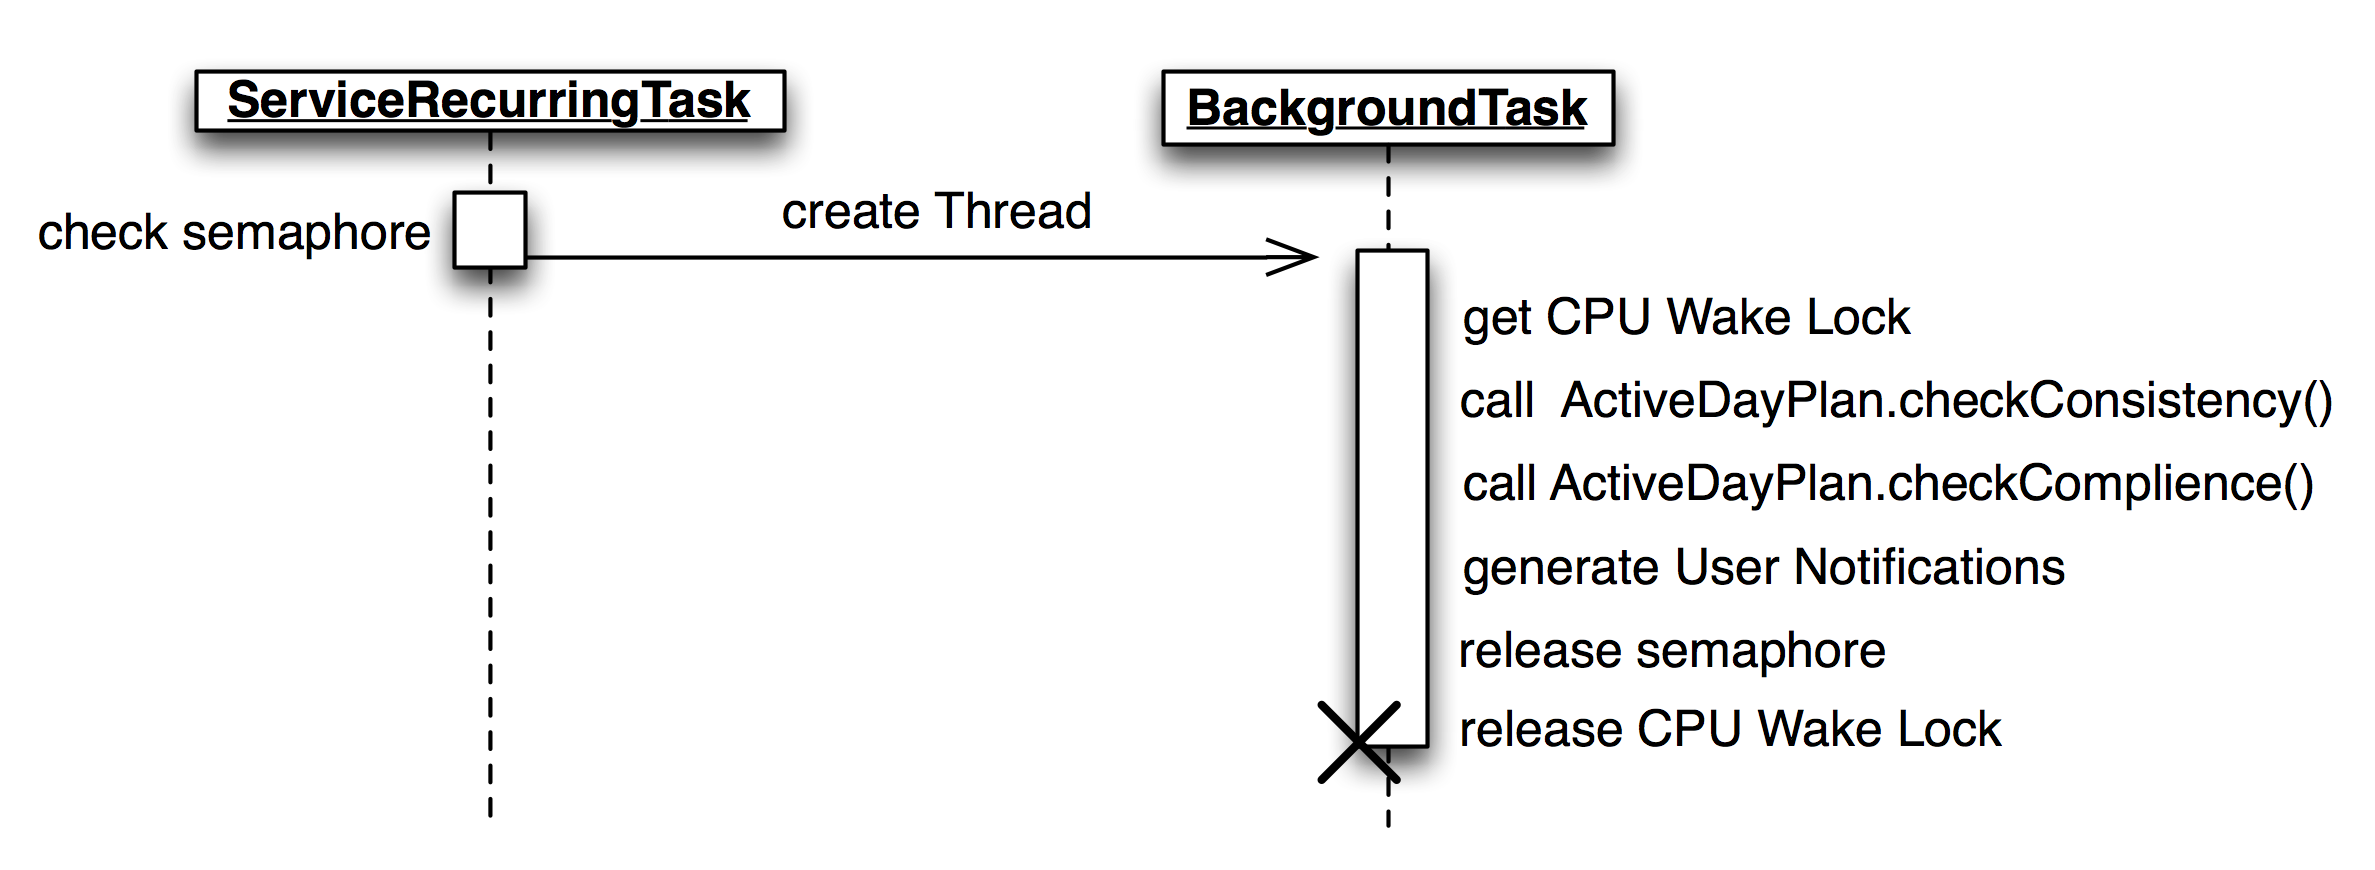
\includegraphics[width=14cm]{pics/background2.png}
\caption{Sequence diagram of the background task}
\label{background2}
\end{figure}  

	
	\subsection{Calendar Integration} % (fold)
	\label{sec:android_calendar}
	All data integration on the Android plattform is done via
so called ``content providers''. These providers are the
only way to transfer data between applications, since there
is no shared space which all applications could use.

However the content provider for the calendar data is
working, but not specified in the official developers
documentation. That means that the API could change at
any time, which has to be considered at the application
design.

In order to not be too dependent on the changing API, a
wrapper layer was built around it. Now there are only four
methods which have to be adapted if the API changes.
\begin{itemize}
  \item queryEvents
  \item insertEventToBackend
  \item updateEventInBackend
  \item deleteEventFromBackend
\end{itemize}

The ``queryEvents'' method can be given a SQL statement as a selection
statement and a String array. Values in the array subsequently replace all
the ``?'' in the statement. The method then returns an ArrayList of
CalendarEvent objects, which suited the selection.

The ``insertEventToBackend'' method is used to insert new events via the
content provider. It takes a CalendarEvent object, builds an Android
ContentValues object from it and inserts this into the backend.

The ``updateEventInBackend'' method does practically the same, but updates
the events in the backend, instead.

At last the ``deleteEventFromBackend'' method removes the passed CalendarEvent
completely from the backend.

These four methods, described above, are the sole fundament of the calendar
wrapper library. As they mostly consist of less than ten lines of code,
the adaption to a new API can be done extremely easily.


	
	\subsection{Introduction of Task management} % (fold)
	\label{sec:android_task}
	TODO: android does not have a task handling/storage

TODO: introduce our task class, explain why constraint-architecture was necessary 

TODO: discuss task serialization 

TODO: storage in calendar, possible different solutions
		
	\newpage
	\subsection{Routing interface (Kangaroo routing framework)} % (fold)
	\label{sub:routing_interface}
	\subsubsection{Classes}

\begin{itemize}

	\item RouteParameter\newline
	\item Place\newline
	\item Vehicle\newline
	\item AmenitySelector\newline
	\item Limits\newline

\end{itemize}

\subsubsection{Methods}

\begin{itemize}

	\item RouteParameter routeTo(Place destination, Vehicle vehicle)\newline
	
	Starting from the current position route to the place definied by destination. The parameter of the fastest route that can be used by the vehicle specified by vehicle will be returned.	
	
	\item RouteParameter routeFromTo(Place start, Place destination, Vehicle vehicle)\newline
	
	Starting from the place definied by start route to the Place definied by destination. The parameter of the fastest route that can be used by the vehicle specified by vehicle will be returned.
	
	\item Place getNearestAmenity(Place position, AmenitySelector selector, Limits limits)\newline

	Starting from the place definied by position find a number of nearest amenity nodes, that fullfil the selection conditions defined by selector und limits. 
	
	\item LocationListener getLocationListener()\newline
	
	

\end{itemize}
	
	\subsection{Routing engine (MobileTSM)} % (fold)
	\label{sub:routing_mobiletsm}
	TODO: review and finalize this chapter\newline
TODO: Andi: check that I divided the routing chapters correctly (generic vs. android specific)\newline

As we already showed, there was no way to get around at least adapting an existing routing engine. As Traveling Salesman is the one to use as a basis, our version of Traveling Salesman implementing the routing interface defined within the Kangaroo routing Framework is called \emph{MobileTSM}. The folling will summarize its structure, explain the most important changes in contrast to the original version of Traveling Salesman and give reasons for the adaptions.

\subsubsection{Main problems arising with decision for TSM}


Coming up with the decision for using Traveling Salesman, there were sseveral issues to work on:

\begin{enumerate}
	\item \textbf{Data storage}
	
		The data storage modules (data sets in Traveling Salesman's terminology) that come with the project can be considered unoptimized or even bad with respect to efficency and performance as needed for a mobile application. There are several different types of data set modules with different approaches of storing and organizing data.\newline
		
		Generally, but on Android's mobile platform in particular, there are two contradictory goals for the data storage architecture. Since Android restricts the heap space for an application to (at this time) 16 megabytes, the map area that can be cached in memory, is limited to several square kilometers, depending of course on data density. Thus one is forced to filter map elements before loading into memory.
		As not only memory is expensive, but also data access to a flash card or a database, a compromise has to be found between loading the whole map into memory and accessing the persistent map database for every single element requested by the routing engine. \newline
		
		TODO: give values
		
	\item \textbf{Routing data}
	
		By default, Traveling Salesman performs every routing operation on the original set of data not dropping elements that do not affect the result of the operation. An example for elements of this type are nodes, that geographically shape the curvature of a street but do not introduce a junction. A node of this type will be called \emph{intermediate way node} and is dispensable for routing operations unless it is the nearest node to the starting or destination point of a route.\newline
		
		Both memory space occupied by the map and time consumption of a routing operation can be reduced by ignoring intermediate way nodes. Nethertheless one cannot dispense with intermediate way nodes close to starting and destination point. This implies an individual routing data set for every routing operation. At first sight this induviduality runs contrary to Traveling Salesman's architecture when aiming at keeping compatibility.\newline		
		
		TODO: give values
											
	\item \textbf{Searching algorithm}
	
		When given two pairs of geographical coordinates and an order to find a route between these two, one has to find the nearest street nodes to starting and destination locations prior to the actual routing operation. This is because non-trivial routing operations can only be performed on a routing graph between vertices. Thus one has to translate from a geographical location to the vertex (node) that best matches it. This can be considered the street node with minimal distance to the given location.\newline
				
		A naive ansatz to finding the nearest street node 	to a geoprahical location would be to iterate over all street nodes, calculate the distance between the location and each street node and select the one with minimal distance. Exactly this is done by Traveling Salesman resulting in an extremly time consuming routing process.\newline
		
		TODO: give values

\end{enumerate}


\subsubsection{Approaches for main problems arising with decision for TSM}

As just explained in the previous section, three main issues have to be handled: reduce and individualize routing data while maintaining compatibility to Traveling Salesman, find an efficient data storage architecture and improve the search algorithm for nearest nodes. The next sections will outline the abstract framework designed to approach these problems.\newline

TODO: still to mention:
\begin{itemize}
	\item filtering intermediate way nodes implies need for an extra field holding distance between street nodes.
	\item derivates of Traveling Salesman's classes \texttt{Node}, \texttt{Way} and \texttt{WayNode}.
\end{itemize}

\subsubsection{Reducing and individualizing of routing data}

The basic idea is to introduce a module, an abstract Java class named \texttt{MobileDataSetProvider}, that can be queried for a specialized set of routing data which is compatible with Traveling Salesman and optimized for an individual routing operation. Any Traveling Salesman router may then be called with a reference to this individual data set. Anyhow, a router can perform another routing operation with different parameters on the same data set, but since the majority of intermediate way nodes will not be included in the data set, it will probably not find the best route or might even fail.\newline

One can also think of adding functionality to recycle an individualized data set. Instead of creating a new one for each routing operation, an old data set may be updated to be as qualified as if it was created specifically for the new parameters. One may be tempted to believe this is the only way to significantly gain time resources, but we will show that in fact our implementation exploits major improvements without this feature.\newline

\subsubsection{Data storage architecture}

The data set provider itself reads data from a suitable data source (for example from database or a file stream). Since even individualized data sets will have a large intersection, data is cached in memory to a great extent.\newline

As an abstraction of the data access to a routing data sources, a Java interface (called \texttt{RoutingDataAdapter}) is introduced. It provides methods to read map elements from a given data source.\newline


\subsubsection{Search algorithm for nearest nodes}

As already demonstrated, the search for the nearest street node is an integral part of a routing operation. Without any assumption about the chronological and geographical pattern of routing operations that will be performed, one has to improve the data structure storing the nodes to be qualified for fast random access. Anyhow, one can think of another way to speed up the search when analyzing the average use.\newline

Besides 


\subsubsection{Routing engine of MobileTSM}

\begin{itemize}
		
	\item Class \texttt{MobileTSMRoutingEngine}
	
		The class \texttt{MobileRoutingEngine} is the \emph{MobileTSM} implementation of a \texttt{RoutingEngine}.
		
	\item Class \texttt{Vehicle}
		
	\item Class \texttt{Limits}

\end{itemize}





	\subsubsection{Tests and benchmarks for MobileTSM}
	\label{sub:routing_testcase}
	In order to test the performance and reliability of the MobileTSM routing engine, we definied a simple test case that tries to cover all routing tasks the routing engine may be faced with when being in "all-day" use.\newline

Consider the following calendar items
\begin{enumerate}
	\item an appointment fixed at a specific position in time and space (latitude/longitude)
	\item a number of variable tasks each based on a special type of amenity (e.g. post box, cash point)
\end{enumerate}

Starting at a point that is in time and space far from the appointment in (1), we make some movements in space which are not necessarily straight into the appointments direction, while time is increasing linearly. At a certain point, the movement turns into a straight movement towards the appointments meeting point. Note that for the movement a single type of vehicle is assumed and it is restricted to an area in space, that is completely covered by the given map file.\newline

Given this movement, the routing engine will be used to periodically perform a set of tasks to give answers to the following questions
\begin{enumerate}
	\item Is there any need to start moving straight to the next appointment? Is there even no way to get there in time anymore?\newline
	Starting from the current position in space, the fastest route to the next\footnote{the one which is in time the next looking from the current time} appointments position in space is calculated. The routing engine will account for the restrictions that are given by the specified vehicle. The time needed to follow this route with the given vehicle is compared to the time that is left until the next appointments meeting time.
	
	\item Is there any way to handle one or more variable task between the current position in time and space and the one given by the appointment in (1) without running the risk of missing this appointment?\newline
	A variable task is selected. Starting from the current position in space, the map is searched for the nearest amenities needed to fullfil the selected task. Given this list of amenities, every\footnote{a more or less intelligent filter should be applied to reduce the list to a minimal number of amenities} single amenity is selected and the following calculations are performed: the fastest route from the current position in space to the selected amenity and the fastest route from this amenity to the next appointments position in space is calculated. Using the sum of the time needed to follow these consecutive routes with the given vehicle and the time needed to fullfil the task is compared to  the time that is left until the next appointments meeting time.
\end{enumerate}

In order to ensure a reproducible  test case, there are some parameters to fix. These are
\begin{itemize}
	\item the map file that containing routing data
	\item the vehicle that is used and hence the infratructure that can be used to get to the destinations
	\item the position in space and time of the appointment in (1), namely time, latitude and longitude
	\item the number and type of variable tasks (including the type of amenity they are based on)
	\item the parameters of the movement previous to the appointment in (1), particularly the starting point in time and space of the movement
\end{itemize}
	
		
		
	\subsection{Routing database} % (fold)
	\label{sub:routing_database}
	
Android comes with an ready-to-use implementation of a SQLite database system which is the one to use in our project to store routing data (cf. chapter \ref{sub:routing_mobiletsm}). It seems reasonable to include all routing data in one database file and to preprocess it in a way that keeps operation expense on the mobile device at a minimum. The follow sections will give details on the database structure and the tools used to convert an Openstreetmap XML to such a database file, including the just mentioned preprocessing.

\subsubsection{Significant map elements for routing data}

The Openstreetmap XML file consists of a set of node, a set of ways and a (for this project dispensable) set of relations. Although in principle every node and way has the same "weight", significance for our application may vary over a huge scale. This significance depends on the attributes of the according map element. Three types of map elements are of high significance:

\begin{itemize}
	\item selected ways
	
		As Openstreetmap also uses ways to map buildings or areas of a special type, public stairways or almost impassable trails, one is forced to drop every way that cannot be considered to be a "standard street"\footnote{we assume the user is not willing to travel such almost impassable trails as a pedestrian}. This selection is based on the tags associated with a way. 
	
	\item selected street nodes
	
		The nodes spanning up a way that wasn't dropped are considered to be significant to our application.\newline
		
		Furthermore, street nodes are (as already mentioned several times) split into two categories. \emph{Intermediate way nodes} may be dropped without any impact on a routing operation traversing the way, whereas \emph{essential street nodes} cannot (cf. chapter \ref{sub:routing_mobiletsm} for details).
		
	\item selected POI\footnote{Point Of Interest} nodes
	
		Nodes that are tagged as an "amenity" or a "shop" of any type are considered to be significant to our application.

\end{itemize}

Note that dropping map elements needs to be done with care to yield a coherent reduced map, since one has to be aware of reciprocal   dependencies between map elements.\newline

\subsubsection{Structure of routing database}

According to the structural demands the database basically consists of four tables:

\begin{itemize}

	\item \texttt{ways\_0}		
						
		Every row in this table represents a way.\newline

		\begin{tabular}[ht]{|p{2.5cm}|p{3.5cm}|p{8.5cm}|}
			\hline
			column & data type & description \\
			\hline\hline
			 id & integer primary key & unique way id (= OSM id)\\
			 name & text not null & name of this way (= OSM 'name' tag)\\	
			 highway & text not null & = OSM 'highway' tag\\
			 maxspeed & integer not null & maximum speed in km/h (= OSM 'maxspeed' tag)\\			 
			 tags & text not null & serialized OSM tags\\
			 flags & integer not null & \emph{unused up to now}\\				 
			 waynodes & text not null & serialized list of way nodes\\
			 waynodes\_red & text not null & serialized list of reduced way nodes\\
			\hline
		\end{tabular}\newline

	
	\item \texttt{street\_nodes\_0}

		Every row in this table represents a street node independently of wether it is an intermediate or an essential way node.\newline

		\begin{tabular}[ht]{|p{2.5cm}|p{3.5cm}|p{8.5cm}|}
			\hline
			column & data type & description \\
			\hline\hline
			 id & integer primary key & unique node id (= OSM id)\\	
			 lat & real not null & latitude of node\\			 
			 lon & real not null & longitude of node\\	
			 tags & text not null & serialized OSM tags\\			 
			 ways & text not null & serialized list of ways connected to this node\\	
			 type & integer not null & type of street node\\				 
			\hline
		\end{tabular}\newline
	
	\item \texttt{poi\_nodes\_0}

		Every row in this table represents a Point Of Interest.\newline
		
		\begin{tabular}[ht]{|p{2.5cm}|p{3.5cm}|p{8.5cm}|}
			\hline
			column & data type & description \\
			\hline\hline
			 id & integer primary key & unique node id (= OSM id)\\	
			 lat & real not null & latitude of node\\			 
			 lon & real not null & longitude of node\\
			 poicode & integer not null & type code of Point Of Interest\\	
			 tags & text not null & serialized OSM tags\\			 
			 nst & integer not null & id of nearest street node\\			 
			\hline
		\end{tabular}\newline
	
	\item \texttt{index}
	
		At the current stage of the project, this table does not contain any crucial data. It is rather intended to be used in future when the map area is split into disjunctive tiles. It then may contain a kind of table of contents.
		
\end{itemize}


\subsubsection{Creation of routing database}
			
	\newpage
	\subsection{Consistency and compliance checks of a day plan} % (fold)
	\label{sub:dayplan}
	Having set up the basic routing toolkit needed to construct a calendar being more intelligent than a standard one, this chapter wants to give details on this additional "intelligence". A calendar in this context is defined to be a list of events and tasks. A calendar is broken into pieces by default covering one day. Although it may in principle cover any period of time, it will be called \emph{day plan}.

\subsubsection{Representation of a day plan (\texttt{DayPlan} class)}

The \texttt{DayPlan} class is a container for events and tasks in the previously explained sense including functionality to operate on its content. Its core component is an algorithm to check whether any arbitrary event in the day plan is compliant with the assumption of "standing" at a fixed but arbitrary location at a fixed but arbitrary time\footnote{the considered event of course has to have a fixed location and start time}. This compliance furthermore depends on the (estimated) existence of the possibility to use a given vehicle to reach the considered event in time.\newline

A compliance check actually tries to find a route starting from the given location to the location of the considered event and returns the time left between the specified time and the start time of the considered event substracted by the estimated time needed to travers the calculated route. Since location and time to start and the event to consider as a target event are free parameters, this algorithm can be used in many ways to be the basis of every use-case.\newline

In fact our application uses an derivate of the \texttt{DayPlan} class, the \texttt{ActiveDayPlan} class, which differ only in the source of tasks and events. While the \texttt{DayPlan} class contains both itself, the \texttt{ActiveDayPlan} will actually access an external calendar via an \texttt{CalendarAccessAdapter}.

\subsubsection{Compliance with current position and time}
 
One question our application is expected to give answer to is \emph{"How much time is left until I have to get going towards my next event to be there in time?"}.\newline

The answer is given by passing the current location (probably the last known GPS location) and the current time to the appropriate method of a \texttt{DayPlan} instance. By definition, the result is the answer to the question, with a negative value indicating an incompliance between the current position and the next event. Thus it can probably not be reached in time. Figure \ref{fig:compliance_check} gives a simplified graphical representation.

\begin{figure}[h!]
	\centering
	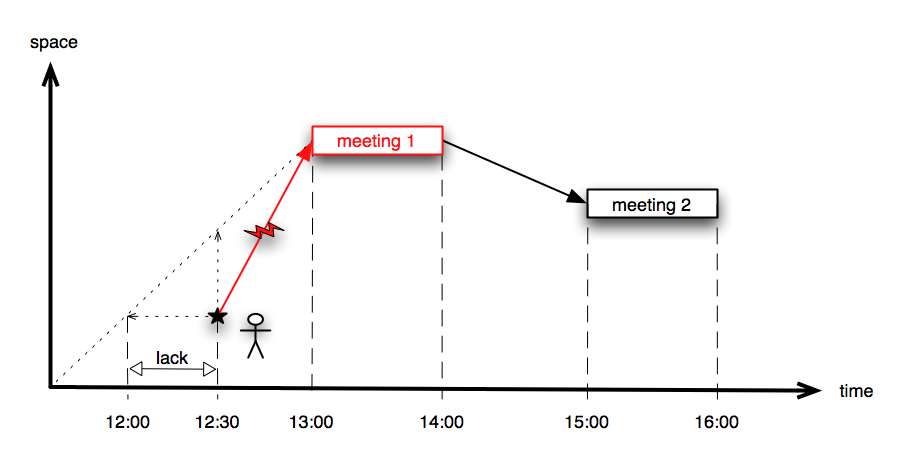
\includegraphics[width=15cm]{pics/compliance_check_lack.png}
	\caption{A conflict revealed by a compliance check: The current position (marked with a stickman) is incompatible with the next event ("meeting 1") since the time needed to get there exceeds the time left. Space is reduced to one dimension for simplicity.}
	\label{fig:compliance_check}
\end{figure}

\subsubsection{Consistency check}

As a day plan probably contains more than one event, it bears potential for inconsistencies in the sense that at least one event cannot be reached in time\footnote{using one single specified vehicle} assuming one adheres to the previous event as fixed in the day plan. The user probably longs to be informed about such inconsistencies. Figure \ref{fig:consistency_check} gives a simplified graphical representation.\newline

A consistency check of a day plan is performed by iteratively checking compliance between one event and its preceeding event and returning a list of conflicts. A conflict can either simply be an incompliance between two subsequent events or any other conflict, including an incapability of finding a route or a temporal overlap between two events.

\begin{figure}[h!]
	\centering
	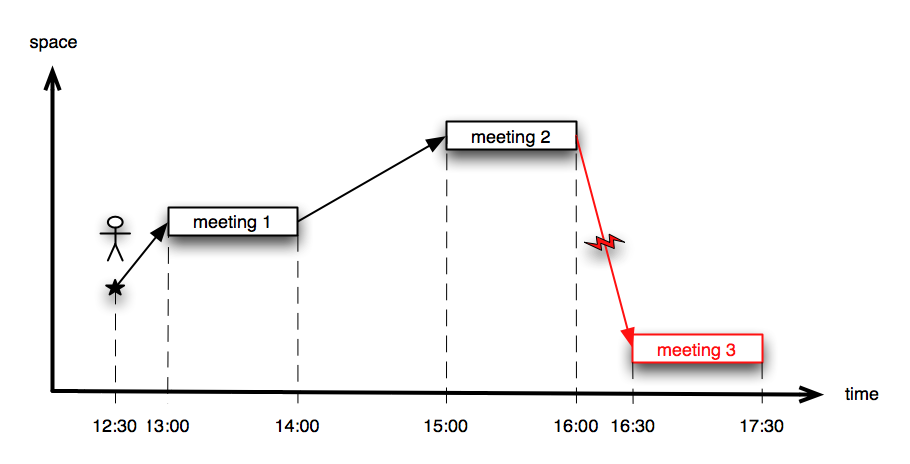
\includegraphics[width=15cm]{pics/consistency_check.png}
	\caption{A conflict revealed by a consistency check: The events "meeting 2" and "meeting 3" are incompatible in the sense that the time needed to from "meeting 2" to "meeting 3" exceeds the time left. Space is reduced to one dimension for simplicity.}
	\label{fig:consistency_check}
\end{figure}









	
			
	\subsection{Optimization of a day plan} % (fold)
	\label{sub:dayplan_optimization}
	TODO: finalize this chapter\newline

Tasks may in principle be considered as events with several parameters, including location and start times, not being fixed. The optimization process of a day plan is defined to try to fix the parameters of the given variable tasks in a desirable way maintaining the day plan's consistency. A task with successfully fixed parameters becomes an event and is thus deleted from the task list and the corresponding event is added to the event list. The task is said to be \emph{fixed as an event} or \emph{executed} within the scope the event.\newline

A task not only has variable parameters to fix but can also have a set of constraints of different types. Task constraints are represented by classes implementing the \texttt{TaskConstraintInterface}. Possible constraints may apply to the date, the day time, the location or several other parameters (see table \ref{tab:dayplan_optimization_constraints} for a complete list task constraints) of the task. The parameters of a task to be fixed as an event have to obey every constraint in the task's constraint set.\newline

The \texttt{DayPlan} class does not perform the optimization itself but allows to set an optimizer that will be used when an optimization process is triggered. An actual optimizer is an implementation of the \texttt{DayPlanOptimizer} interface.\newline

	\begin{tabular}[ht]{|p{4.5cm}|p{8.5cm}|}
		\hline
		name & description \\
		\hline\hline
		\texttt{TaskConstraintDate} & specifies an end and/or a start date\\
		\texttt{TaskConstraintDayTime} & specifies an end and/or a start day time\\
		\texttt{TaskConstraintDuration} & specifies the time needed to execute the task\\
		\texttt{TaskConstraintLocation} & specifies a location the task has to be executed at\\
		\texttt{TaskConstraintPOI} & specifies a type of a Point Of Interest the task needs to be executed\\	
		\hline
	\end{tabular}\newline

\subsubsection{Approaches to optimization}
 
"Optimization" implies the need for a measure of some kind of quality. Optimization then is the process of finding the solution of highest quality. The most desirable way of optimizing a day plan is to input a day plan (consisting of events and tasks) and a measure of quality (metric) into a black box algorithm returning the best day plan possible maintaining day plan consistency. Since this is probably one of the most challanging problems in computer science, we are forced to make strong simplifications and accept the fact that the solution is likely to be not the optimal one.\newline

Our basic approach to this problem is to use a greedy algorithm recursively trying to fix tasks between the events of a day plan, implemented in the class \texttt{GreedyTaskInsertionOptimizer}. The optimization is started specifying a location, a time and a vehicle where the location and the time are used as a starting point. The algorithm iterates over the list of tasks in the order given by a \texttt{TaskPriorityComparator}. For every task, it consecutively checks compatibility between the constraints associated with the task and the parameters it is potentially fixed with. These potential parameters are determined based on the specified starting point (location and time) and the task's constraints.\newline

TODO: give a short explanation of parameter determination\newline

The first task that fulfills every constraint is fixed as an event and the optimization process is started recursively with the recently fixed end time and location of the task.

\subsubsection{Implementations of a \texttt{TaskPriorityComparator}}

			
	\subsection{Persistent Storage} % (fold)
	\label{sec:android_pers_storage}
	For persistent database storage, the Android API contains
support for SQLite databases. Any application can create
an SQLite object, which is stored on the device under
``/data/data/package\_name/databases''

Unfortunately, up to Android version 2.1, the installed
support for SQLite is 2.5.9. This means that it is not
possible to benefit from the support for $R^*$-Trees,
which was included in SQLite 2.6. This would have meant
a very comfortable way of storing location data and
retrieving positions in vincinity of a given point.


%conclusion and future work	
\chapter{Conclusion and future Work} % (fold)
\label{chp:platform_choice}
\section{Accomplishments}
\label{sec:accomplishments}
\subsubsection{Application for optimized dayplans} % (fold)
\label{ssub:Application for optimized dayplans}
Several goals were accomplished while working on this teamproject. First of all
an application was created which supports a users day planning with the
following implemented functionalities:
\begin{itemize}
  \item Generate a dayplan, which is heavily optimized on completing as many
    tasks as possible
  \item Simple, yet powerful task management system
  \item Enter location data for any event in the calendar
  \item Full integration with Android calendar infrastructure
  \item Routing between events supporting a variety of time and space
    constraints
  \item Continous checking of the dayplan's consistency and compliance
  \item Notification of the user for every event and deadline according to the
    dayplan
\end{itemize}


\subsubsection{Easily reusable Open Source packages} % (fold)
\label{ssub:Easily reusable Open Source packages}
Additionally to the functionality, many parts of the application's structure can
be easily reused in other projects.

\paragraph{Calendar Library}
The calendar library provides an easy interface to query calendar data from the
Android platform. The queried data is then easily accessible via Java objects
and can be used in any Java application for Android. It can even be adapted to
other platforms with very small amount of adaptions to the library.

\paragraph{Routing Engine}
The routing engine underlying the kangaroo application is a fully self-contained
java package. It can be easily reused for routing purposes in any Java
application which needs to access Open Streetmap data.

\paragraph{Task Manager}
The task management functionality of kangaroo is also strongly encapsulated and
can therefore be reused easily in any Java project. The storage mechanism of
converting tasks into events and storing them at a specific date can also be
adapted easily to an SQLite database or any other preferred storage solution

\paragraph{Dayplan}
The Dayplan class as the centre of the whole application is also only loosely
coupled with the rest of the application. This means as it is also a pure Java
package, it can be reused easily and any other routing engine, calendar library,
task manager and user interface can be simply connected to the dayplan. Thus
providing the kangaroo functionality in a whole different environment and not
only on the android platform.

\subsubsection{Personal Experience} % (fold)
\label{ssub:Personal Experience}
Last but not least, a whole lot of knowledge was gained during the development
of kangaroo. At the beginning none of the developers was familiar with
developing applications for the Android platform. During the last months however
a huge knowledge was accumulated, including structure, optimization and
architecture of simple up to advanced applications for one of the big rising
mobile platforms.

% subsubsection Personal Experience (end)

\section{What to do differently} % (fold)
\label{sec:Whattododifferently}
\subsubsection{Milestones} % (fold)
\label{ssub:Milestones}

% subsubsection Milestones (end)
\subsubsection{Unit tests} % (fold)
\label{ssub:Unittests}
Early in the development process we decided to not do unit tests.
At the time there were several reasons for that.
As the routing engine and the calendar integration were the first
things to be developed, they were crucial in the decision process.
Unit testing on the Android platform seemed rather complicated,
especially for code using the content provider backend. In a discussion
with our advisor, we decided that it would be too time consuming,
considering how much time already had passed for specification and
platform choosing. Therefore we decided to concentrate the time left
on actual development.

However, we had several situation in the development process, where
unit testing would have been useful. Many problems only became
apparent when certain elements were integrated together. Unit tests
could have revealed these much earlier. Especially as we developed
on our own much more often than anticipated. This accounted for more
problems whilst integrating, which could also have been minimized by
unit testing.

% subsubsection Unit tests (end)

\subsubsection{Bug tracker} % (fold)
\label{ssub:Bugtracker}
Although a bug tracker is provided by github, we didn't use it
until the very end of the project. In retrospect it would have been
better to utilize the bug tracker right from the start. This would
have forced us to look deeper into bugs and better document them, if
similar bugs appeared later.

Especially in combination with unit tests the bug tracker could have
improved the development process significantly. A good approach, for
example, would have been, to create a unit test for every occurring bug.
This means that there is an immediate way to test if the bug was
fixed and that it would not be introduced again later.

% subsubsection Bug tracker (end)
% section What to do differently (end)
\section{Future work}
As future projects, one can imagine many fields, not only directly concerning
the kangaroo application. Of course, some minor adjustments have to be done to
kangaroo, if it should be ready to be deployed via the Android market. The UI
could be polished a bit to match the design of modern mobile applications.
Additionally some system parts can be improved, mainly in the area of routing
performance, to guarantee a smother and faster experience for the end user.

Nevertheless one of the big strengths of the kangaroo project are definitely the
amount of easily, reusable Java packages. As the whole code is open sourced, all
parts can be used to build other routing related applications. But also
integrate with calendar data, build an improved task management application or
port the Dayplan optimizing functionality to another routing engine like Google
Maps for example.


%\bibliographystyle{include/splncs}
%\bibliography{include/literatur}

\end{document}
